\documentclass[12px, a4paper]{article}
\usepackage[utf8]{inputenc}
% ~~~~~~~~~~~~~~~~~~~~~~~~~~~~~~~~~~~~~~~~~~~~~~~~~~~~~~~~~~~~~~~~~~~~~~~~~~~~~~
% Packages to be loaded before others
% ~~~~~~~~~~~~~~~~~~~~~~~~~~~~~~~~~~~~~~~~~~~~~~~~~~~~~~~~~~~~~~~~~~~~~~~~~~~~~~
\input{preamble/preamble_commands}
% Calculation with LaTeX
\usepackage{calc}
% Language setting
\usepackage[ngerman]{babel}
% Colors
\usepackage{xcolor}
% Graphics
\usepackage{graphicx}



% ~~~~~~~~~~~~~~~~~~~~~~~~~~~~~~~~~~~~~~~~~~~~~~~~~~~~~~~~~~~~~~~~~~~~~~~~~~~~~~
% Fonts
% ~~~~~~~~~~~~~~~~~~~~~~~~~~~~~~~~~~~~~~~~~~~~~~~~~~~~~~~~~~~~~~~~~~~~~~~~~~~~~~
\usepackage[T1]{fontenc}
% Additional Symbols (Text Companion font extension)
\usepackage{textcomp}



% ~~~~~~~~~~~~~~~~~~~~~~~~~~~~~~~~~~~~~~~~~~~~~~~~~~~~~~~~~~~~~~~~~~~~~~~~~~~~~~
% Math
% ~~~~~~~~~~~~~~~~~~~~~~~~~~~~~~~~~~~~~~~~~~~~~~~~~~~~~~~~~~~~~~~~~~~~~~~~~~~~~~
\usepackage{amsmath}



% ~~~~~~~~~~~~~~~~~~~~~~~~~~~~~~~~~~~~~~~~~~~~~~~~~~~~~~~~~~~~~~~~~~~~~~~~~~~~~~
% Symbols
% ~~~~~~~~~~~~~~~~~~~~~~~~~~~~~~~~~~~~~~~~~~~~~~~~~~~~~~~~~~~~~~~~~~~~~~~~~~~~~~
%%% for Math
%\usepackage{mathrsfs} %% Schreibschriftbuchstaben für den Mathematiksatz (nur Großbuchstaben)
%\usepackage{dsfont}   %% Double Stroke Fonts
%\usepackage[mathcal]{euscript} %% adds euler mathcal font
\usepackage{amssymb}
%\usepackage[Symbolsmallscale]{upgreek} % upright symbols from euler package [Euler] or Adobe Symbols [Symbol]
%\usepackage[upmu]{gensymb}             % Option upmu
%%% common
%\usepackage{wasysym}  %% Doc: http://www.ctan.org/tex-archive/macros/latex/contrib/wasysym/wasysym.pdf
%\usepackage{marvosym} %% Symbols from marvosym Font
%\usepackage{pifont}   %% ZapfDingbats



% ~~~~~~~~~~~~~~~~~~~~~~~~~~~~~~~~~~~~~~~~~~~~~~~~~~~~~~~~~~~~~~~~~~~~~~~~~~~~~~
% Text
% ~~~~~~~~~~~~~~~~~~~~~~~~~~~~~~~~~~~~~~~~~~~~~~~~~~~~~~~~~~~~~~~~~~~~~~~~~~~~~~
%%% Refs
\usepackage[ngerman]{varioref}
\usepackage{hyperref}
%%% Columns
\usepackage{multicol}



% ~~~~~~~~~~~~~~~~~~~~~~~~~~~~~~~~~~~~~~~~~~~~~~~~~~~~~~~~~~~~~~~~~~~~~~~~~~~~~~
% Graphics
% ~~~~~~~~~~~~~~~~~~~~~~~~~~~~~~~~~~~~~~~~~~~~~~~~~~~~~~~~~~~~~~~~~~~~~~~~~~~~~~
\usepackage[all]{xy}
\usepackage{float}
\usepackage{tikz}
%%% Doc: ftp://tug.ctan.org/pub/tex-archive/macros/latex/contrib/subfig/subfig.pdf
% Incompatible: loads package capt-of. Loading of 'capt-of' afterwards will fail therefor
\usepackage{subfig}



% ~~~~~~~~~~~~~~~~~~~~~~~~~~~~~~~~~~~~~~~~~~~~~~~~~~~~~~~~~~~~~~~~~~~~~~~~~~~~~~
% Captions & Style
% ~~~~~~~~~~~~~~~~~~~~~~~~~~~~~~~~~~~~~~~~~~~~~~~~~~~~~~~~~~~~~~~~~~~~~~~~~~~~~~
%%% Doc: ftp://tug.ctan.org/pub/tex-archive/macros/latex/contrib/caption/caption.pdf
\usepackage{caption}
% Aussehen der Captions fuer subfigures (subfig-Paket)
\IfPackageLoaded{subfig}{
    \captionsetup[subfloat]{%
        margin = 10pt,
        font = {small,rm},
        labelfont = {small,bf},
        format = plain, % oder 'hang'
        indention = 0em,  % Einruecken der Beschriftung
        labelsep = space, %period, space, quad, newline
        justification = RaggedRight, % justified, centering
        singlelinecheck = true, % false (true=bei einer Zeile immer zentrieren)
        position = bottom, %top
        labelformat = parens % simple, empty % Wie die Bezeichnung gesetzt wird
    }
}



% ~~~~~~~~~~~~~~~~~~~~~~~~~~~~~~~~~~~~~~~~~~~~~~~~~~~~~~~~~~~~~~~~~~~~~~~~~~~~~~
% Misc
% ~~~~~~~~~~~~~~~~~~~~~~~~~~~~~~~~~~~~~~~~~~~~~~~~~~~~~~~~~~~~~~~~~~~~~~~~~~~~~~
% Theorems
\usepackage{amsthm}
\newtheorem{Definition}{Definition}
\newtheorem{Beispiel}{Beispiel}
\newtheorem{Satz}{Satz}
\newtheorem{Bemerkung}{Bemerkung}
\newtheorem{Algorithmus}{Algorithmus}
\newtheorem{Lemma}{Lemma}
% Listings
\usepackage{listings}
\definecolor{Brown}{cmyk}{0,0.81,1,0.60}
\definecolor{OliveGreen}{cmyk}{0.64,0,0.95,0.40}
\definecolor{CadetBlue}{cmyk}{0.62,0.57,0.23,0}
\definecolor{lightlightgray}{gray}{0.9}
\lstset{
    language=C,                             % Code langugage
    basicstyle=\rm\ttfamily,                % Code font, Examples: \footnotesize, \ttfamily
    keywordstyle=\color{OliveGreen},        % Keywords font ('*' = uppercase)
    commentstyle=\color{gray},              % Comments font
    numbers=left,                           % Line nums position
    numberstyle=\tiny,                      % Line-numbers fonts
    stepnumber=1,                           % Step between two line-numbers
    numbersep=5pt,                          % How far are line-numbers from code
    backgroundcolor=\color{lightlightgray}, % Choose background color
    frame=none,                             % A frame around the code
    tabsize=2,                              % Default tab size
    captionpos=b,                           % Caption-position = bottom
    breaklines=true,                        % Automatic line breaking?
    breakatwhitespace=false,                % Automatic breaks only at whitespace?
    showspaces=false,                       % Dont make spaces visible
    showtabs=false,                         % Dont make tabls visible
    %columns=flexible,                       % Column format
    %morekeywords={someword, otherword},     % specific keywords
}

\usepackage{amsmath}
\usepackage{hyperref}
\usepackage{float}
\usepackage{algorithm}
\usepackage{arevmath}     % For math symbols
\usepackage[noend]{algpseudocode}

\begin{document}
\setlength{\parindent}{0em}
%front
\input{content/00_title}
%Einfügen des Inhaltsverzeichnisses
\tableofcontents
\newpage
\thispagestyle{empty}
\mbox{}\thispagestyle{empty}
\newpage
%main

\section{Vorwissen und Konventionen}

\subsubsection*{Differenzierbarkeit reeller Funktionen} 
Eine reelle Funktion $f : (a, b) \to \mathbb{R}$  heißt differenzierbar in $x \in (a,b)$, falls der Grenzwert $\lim_{h \to 0}  \frac{f(x +h) - f(x)}  {h}$ existiert. In diesem Fall heißt dieser Grenzwert die Ableitung (Steigung) von $f$ in $x$ und wird mit $f' (x)$ bezeichnet.
\begin{figure}[H]
      \centering
    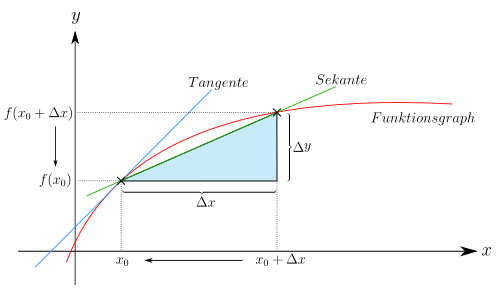
\includegraphics[width=0.8\textwidth]{images/Differencial_quotient_of_a_function}
      \caption{Quelle: Wikipedia: https://de.wikipedia.org/wiki/Datei:Differencial\_quotient\_of\_a\_function.svg}
\end{figure}

\subsubsection*{Mittelwertsatz einer Veränderlichen} 

Sei $f : [a,b] \to \mathbb{R}$ stetig und differenzierbar für alle $x \in (a,b)$. Dann gibt es $\xi \in (a,b)$ mit
$f'(\xi) = \frac{f(b) - f(a)} { b-a}$.
\begin{figure}[H]
      \centering
    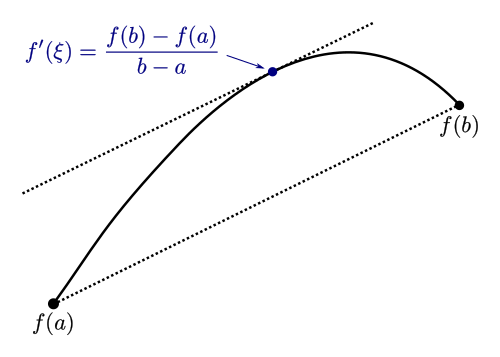
\includegraphics[width=0.6\textwidth]{images/Mittelwertsatz3.png}
      \caption{Quelle: Wikipedia: https://commons.wikimedia.org/wiki/File:Mittelwertsatz3.svg}
\end{figure}

\subsubsection*{Taylorapproximation einer Veränderlichen} 

Jede  reelle Funktion $f$, deren $p+1$-ten Ableitungen existieren und stetig sind lässt sich mit Hilfe der Taylorreihe  $$f(x) = f(a) + f^{'}(a) (x-a) +   \frac{1}{2!} f^{''}(a) (x-a)^2 + \cdots  +  \frac{1}{p!} f^{(p)}(a) (x-a)^{p} +  R_{p+1}(x,a) $$
und dem Restglied  $R_p(x,a) :=   \frac{1}{(p+1)!} f^{(p+1)}(\xi) (x-a)^{p} $ mit einem $\xi \in (x,a)$ darstellen.


\subsubsection*{Cauchy-Schwarzsche Ungleichung}
 Für zwei Vektoren $v,w \in \mathbb{R}^n$ gilt: 
\begin{align*}
\frac{\langle v, w \rangle}{||v|| \cdot ||w||} = \cos(\varphi) 
\end{align*}
wobei $\varphi$ der Innenwinkel zwischen $v$ und $w$ ist.

\subsubsection*{Äquivalenz von Normen}
 Die Normen $||v||: = \sqrt{\sum_{i = 1}^n v_i^2}$ und $||v||_{\infty}:= \max \{ v_1, \cdots, v_n \} $ sind Äquivalent. Sie lassen sich  mit Konstanten $k_1 ||v|| < ||v||_{\infty} k_2  ||v|| $ gegeneinander abschätzen.

\subsubsection*{Symmetrische Matrizen}
 Für eine symmetrische Matrix $A \in \mathbb{R}^{n \times n}$ ist Äquivalent:
\begin{itemize}
\item $A$ hat positive Eigenwerte.
\item $v^TA v > 0$ für alle $v \neq 0$.
\item alle Unterdeterminanten sind positiv. Speziell für $n=2$ und $A = \begin{pmatrix} a & b \\ b & d\end{pmatrix}$ bedeutet dies
$a >0$ und $ad -b^2 >0$. 
\end{itemize}

\begin{Definition}[Konventionen]
In diesem Abschnitt ist $U \subset \mathbb{R}^n$ stets eine offene Teilmenge des $\mathbb{R}^n$.
 $e_i := \begin{pmatrix}  0 \\  \vdots \\ 1  (\text{i-te Zeile})\\ \vdots \\ 0 \end{pmatrix}$  bezeichnet den $i$-ten Basisvektor des $\mathbb{R}^n$.

\end{Definition}

\section{Mehrdimensionale Differentialrechnung}

\begin{Definition}[Konvergenz]
 Eine Folge $(a_n)$ in $\mathbb{R}^n$ heißt konvergent gegen den Grenzwert $a \in \mathbb{R}^n$, wenn gilt:
\begin{align*}
\forall {\varepsilon > 0} \ \exists \ N \in \mathbb{N} \; \forall \ n > N: \; d(a, a_n) < \varepsilon\,
\end{align*}
In Worten: Es gibt für jedes beliebige (noch so kleine) $\varepsilon$ einen Index $N$ derart, dass für alle Indizes $n > N$, also alle weiteren Folgenglieder, gilt: Der Abstand $d(a, a_n)$ ist kleiner als $\varepsilon$.
\end{Definition}

\begin{figure}[H]
      \centering
    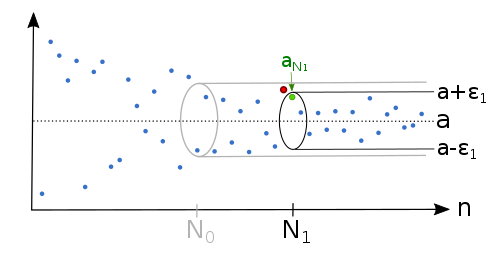
\includegraphics[width=0.9\textwidth]{images/500px-Epsilonschlauch_klein}
      \caption{Quelle: Wikipedia: https://commons.wikimedia.org/wiki/File:Epsilonschlauch\_klein.svg}
\end{figure}



\begin{Definition}[Grenzwert]
Sei $f :X \subset \mathbb{R}^n \to \mathbb{R}^m$ eine  Funktion und $a \in X$. Wir nennen $L_a \in \mathbb{R}^m$ Grenzwert von $f$ bezüglich der Annäherung von $x$ an $a$, falls für jede  konvergente Folge $x_n \to a$  die Folge $f(x_n)$ nach $L_a$ konvergiert.  In diesem Fall bezeichnen wir
\begin{align*}
\lim_{x \to a} f(x) = L_a \;.
\end{align*}
Dies ist gleichbedeutend damit, dass für jedes $\epsilon > 0$ ein $\delta > 0$ existiert, so dass
$d(f(x) ,L_a) < \epsilon$ gilt für jedes $x$ mit $d(x, a) < \delta$.
\end{Definition}


\begin{figure}[H]
      \centering
    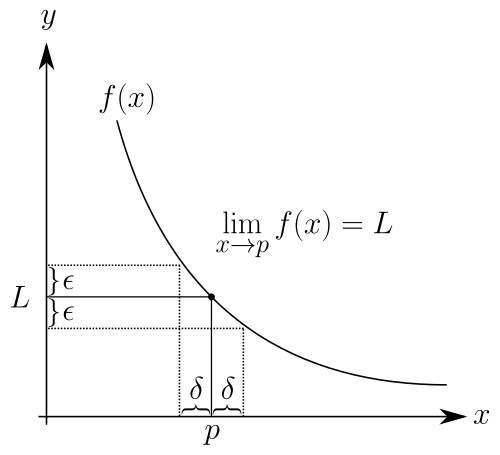
\includegraphics[width=0.6\textwidth]{images/500px-Limes_Definition_Vektorgrafik}
      \caption{Quelle: Wikipedia: https://de.wikipedia.org/wiki/Datei:Limes\_Definition\_Vektorgrafik.svg}
    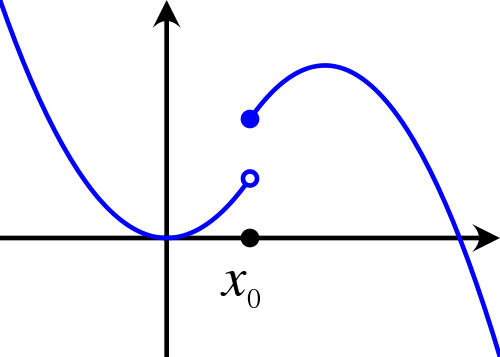
\includegraphics[width=0.6\textwidth]{images/500px-Upper_semi}
      \caption{Quelle: Wikipedia: https://commons.wikimedia.org/wiki/File:Upper\_semi.svg}
\end{figure}




\begin{Definition}[Stetige Funktion]
Eine reellwertige Funktion $f :U \to \mathbb{R}$ heißt stetig, wenn für alle $y \in U$ der Grenzwert $\lim_{x \to y} f(x) = L_{y} $ existiert.
\end{Definition}


\subsection{Richtungsableitung und Gradient reellwertiger Funktionen}
Ableitungen beschreiben bildlich gesprochen das Verhalten einer Funktion bezüglich beliebig kleiner Änderungen der Eingabewerte.





\begin{Definition}[Richtungsableitung]
Sei $f: U \to \mathbb{R}$ eine Funktion. Für einen Vektor $h \in  \mathbb{R}^n$, $t \in \mathbb{R}$  und einen Punkt  $a \in U$ heißt der Grenzwert (falls er existiert) 
\begin{align*}
\partial_h f(a) := \lim_{t \to 0} \frac{f(a + th) - f(a)}{t}
\end{align*}
Richtungsableitung von $f$ am Punkt $a$ in Richtung $h$. Sie misst die Änderung der Funktion in Richtung $h$.

Speziell nennen wir für die Standard Basisvektoren $e_i$ 
\begin{align*}
\frac{\partial f(a)}{\partial x_i}  := \partial_{e_i} f(a) := \lim_{t \to 0} \frac{f(a + t e_i) - f(a)}{t}
\end{align*}
die partielle Ableitung von $f$ in $a$ nach $x_i$.
\end{Definition}

\begin{Definition}[Partielle Differenzierbarkeit]
Eine Funktion  $f: U \to \mathbb{R}$ heißt partiell differenzierbar im Punkt $a \in U$, falls alle partiellen Ableitungen 
$$\frac{\partial f(a)}{\partial x_1}, \cdots , \frac{\partial f(a)}{\partial x_n}$$ 
existieren.
\end{Definition}

\begin{Definition}[Differenzierbarkeit]
\label{diffbarkeit}
Eine Funktion $f: U \to \mathbb{R}$ heißt  differenzierbar im Punkt $a \in U$, falls alle partiellen Ableitungen 
$$\frac{\partial f(a)}{\partial x_1}, \cdots, \frac{\partial f(a)}{\partial x_n}$$
 existieren und stetig sind.  Mann nennt  in diesem Fall die $1 \times n$-Matrix 
$$df(a) := \biggl( \frac{\partial f(a)}{\partial x_1}, \cdots, \frac{\partial f(a)}{\partial x_n} \biggr)$$
das Differential von $f$ im Punkt $a$. Der Vektor 
$$\nabla f (a) := \begin{pmatrix}  \frac{\partial f(a)}{\partial x_1} \\  \vdots \\ \frac{\partial f(a)}{\partial x_n}  \end{pmatrix}$$
wird als Gradient bezeichnet. Es ist $df(a) \cdot h = \langle \nabla f (a) , h \rangle$.
\end{Definition}

\fbox{\parbox{\linewidth}{
$\star \star \bigstar $  Der Unterschied zwischen  Differenzierbarkeit und partieller Differenzierbarkeit ist also, dass die partiellen Ableitungen zusätzlich  zur Existenz auch stetig sein müssen.
}}

\begin{figure}[H]
      \centering
    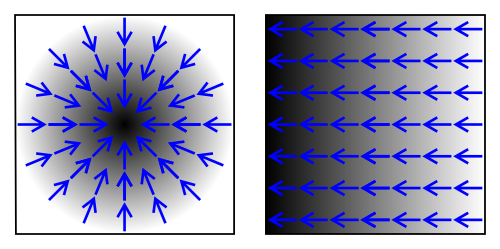
\includegraphics[width=1.0\textwidth]{images/Gradient}
      \caption{Quelle: Wikipedia: https://commons.wikimedia.org/wiki/File:Gradient2.svg}
\end{figure}


\begin{Bemerkung}
\label{partial1}
Für das Differential einer differenzierbaren Funktion  $f: U \to \mathbb{R}$ gilt für alle $a \in U$:
\begin{itemize}
\item  $df(a) (h) :=  df(a) \cdot h$ ist eine lineare Abbildung von $\mathbb{R}^n$ nach $\mathbb{R}$.
\item $df(a)  \cdot h = \partial_h f(a)$. 
\item $d (f \cdot g) = g(a) d(f) + f(a) dg$
\item $d(f + g) = df + dg$
\end{itemize}
\end{Bemerkung}
\begin{proof}
\begin{itemize}
\item  Multiplikation mit einer Matrix ist eine lineare Abbildung.
\item Für die Basisvektoren ist per Definition $df(a)  \cdot e_i = \partial_{e_i} f(a)$. Da jeder Vektor $h$ eine Linearkombination der Basisvektoren ist und $df$ linear ist, folgt die Behauptung.
\item Folgt direkt aus der entsprechenden Eigenschaft reeller Funktionen.
\item Folgt direkt aus der entsprechenden Eigenschaft reeller Funktionen.
\end{itemize}
\end{proof}


\begin{Satz}[Steilste Anstiegsrichtung]
Sei   $f: U \to \mathbb{R}$ differenzierbare Funktion,  $a \in U$ und $v := \text{argmax}_{ h \in S^n} \partial_h f(a) $.
Dann gilt 
\begin{align*}
|| \nabla f(a) || v =  \nabla f(a) \; .
\end{align*} 
\end{Satz}
\begin{proof}
Mit der CSU Ungleichung folgt für beliebiges $h$ 
\begin{align*}
\partial_h f(a) = df(a) h = \langle \nabla f(a) , h \rangle = || \nabla f(a)||  \cdot ||h|| \cdot \cos(\varphi) 
\end{align*} 
wobei $\varphi$ den Innenwinkel zwischen $\nabla f(a)$ und $h$ bezeichnet. Für $||h|| = 1$ wird somit $\partial_h f(a) $ maximal, wenn $\varphi = 0$ und somit $h =  \frac{\nabla f(a)}{||\nabla f(a)||}$ ist.
\end{proof}





%-----------------------------------------------------
% Ende VL 1
%-----------------------------------------------------


\begin{Satz}[Lokale Linearisierung]
\label{lokaleLinearisierung}
Ist  $f: U \to \mathbb{R}$ differenzierbar, so gibt es ein Restglied $R(h)$ mit  $\lim_{h \to 0} \frac{R(h)}{ ||h||} = 0$  so dass für alle $a \in U$ und $h \in \mathbb{R}$ 
\begin{align*}
f(a + h)  =  f(a)  +  df(a) \cdot h + R(h) 
\end{align*}
gilt. 
\end{Satz}

\fbox{\parbox{\linewidth}{
$\star \star \bigstar $ Eine differenzierbare Funktion kann  auf hinreichend kleinen Umgebungen  \\
beliebig genau durch eine lineare Funktion approximiert werden. 
}}

\fbox{\parbox{\linewidth}{
$\diamond \Diamond $  Der Beweis beruht im Wesentlichen auf dem Mittelwertsatz einer Veränderlichen.
}}


\begin{proof}
Wir wählen einen offenen, achsenparallelen Quader $Q \subset U$, so dass er vollständig in $U$ enthalten und $a \in Q$ ist.
Jeder Punkt $a + h \in Q$  lässt sich damit durch einen achsenparallelen Streckenzug durch die Punkte
\begin{align*}
& a_0 := a \\
& a_i  := a_{i-1} + h_i e_i;  \;  \;  i = 1, \cdots , n
\end{align*} 
mit $a$ verbinden. 
\begin{figure}[H]
      \centering
    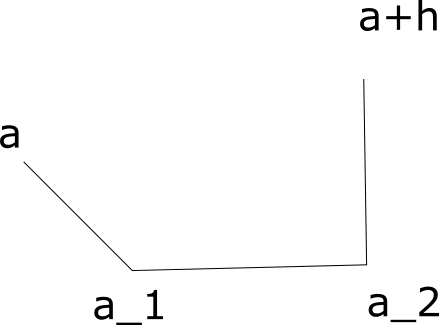
\includegraphics[width=0.4\textwidth]{images/kantenzug}
      \caption{Kantenzug mit achsenparallelen Kanten}
\end{figure}

Damit ist $f(a + h) - f(a) = \sum_{i=1}^{n} \bigl( f (a_i)   - f(a_{i-1})   \bigr)$ und  mit $\varphi_i(t) : = f(a_i + t e_i)$ gilt 
$f(a_i) - f(a_{i-1}) = \varphi_i(h_i)  - \varphi_i(0)$. Wegen dem Mittelwertsatz einer Veränderlichen gibt  es  $\tau_i$  mit
\begin{align*}
\varphi_i(h_i)  - \varphi_i(0)  = h_i \varphi'(\tau_i) \;.
\end{align*} 
Da $\varphi'_i(t) = \frac{\partial  f(a_{i-1} + t e_i ) }{\partial x_i}$ folgt mit $\xi_i: = a_i + \tau_i e_i$ 

\begin{align*}
f(a + h) - f(a) - df(a) \cdot h = \sum_{i=1}^n  \biggl( \frac{\partial  f(\xi) }{\partial x_i} -    \frac{\partial  f(a) }{\partial x_i}   \biggr) h_i
\end{align*} 
und damit
\begin{align*}
| f(a + h) - f(a) - df(a) \cdot h |  \leq || h ||_{\infty}  \sum_{i=1}^n  \biggl| \frac{\partial  f(\xi) }{\partial x_i} -    \frac{\partial  f(a) }{\partial x_i}   \biggr | \; . 
\end{align*} 
Für $h \to 0$ gilt $\xi_i \to a$ und da die partiellen Ableitung stetig sind nach Voraussetzung und alle Normen äquivalent sind folgt

\begin{align*}
\lim_{h \to 0} \frac{ f(a + h) - f(a) - df(a) \cdot h}{||h||} = 0 
\end{align*} 
und damit die Behauptung.
\end{proof}

\begin{Bemerkung}
\label{differentialeindeutig}
Umformuliert bedeutet Satz \ref{lokaleLinearisierung}, dass für das Differential einer differenzierbare Funktion
\begin{align}
\lim_{h \to 0} \frac{f(a + h) -f(a) - df(a) h }{||h||} = 0
\end{align}
Ist $L$ eine weiter lineare Abbildung mit $\lim_{h \to 0} \frac{f(a + h) -f(a) - L(a) h }{||h||}$, so ist $L = df$. Das Differential ist somit eindeutig durch die Eigenschaft der lokalen Linearisierung bestimmt.
\end{Bemerkung}
\begin{proof}
Für $v \in \mathbb{R}^n$ mit $||v|| = 1$ gilt 
\begin {align*}
\bigl( L(a) - df(a) \bigr)(v) =  \lim_{t \to 0}  \bigl( L(a) - df(a) \bigr) \bigl( \frac{tv}{||tv||} \bigr) = \lim_{t \to 0} \frac{\bigl( L(a) - df(a) \bigr)(tv) }{||tv||} = 0
\end{align*}
Da jeder Vektor als Linearkombination von Einheitsbasisvektoren dargestellt werden kann, folgt die Behauptung.
\end{proof}

\begin{Definition}[Differenzierbarer Weg]
Seien $a,b \in \mathbb{R}$. Ein Weg ist eine Abbildung  
\begin{align*}
& \gamma:  [a,b] \to \mathbb{R}^n \\
& \gamma (t) :=  \begin{pmatrix} \gamma_1(t) \\ \vdots \\ \gamma_n(t) \end{pmatrix}
\end{align*}
mit reellen, stetigen Funktionen $y_i : [a,b] \to \mathbb{R}$ (damit ist auch $\gamma$ stetig). Der Weg heißt differenzierbar, falls alle Ableitungen $\gamma_i'(t)$ existieren. In diesem Fall definieren wir
\begin{align*}
 \gamma' (t) :=  \begin{pmatrix} \gamma'_1(t) \\ \vdots \\ \gamma'_n(t) \end{pmatrix}
\end{align*}
\end{Definition}

\begin{figure}[H]
      \centering
    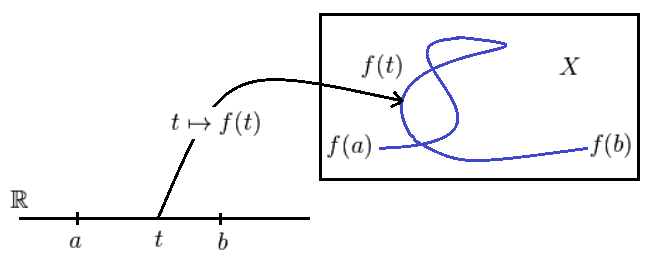
\includegraphics[width=0.8\textwidth]{images/EbeneKurve}
      \caption{Quelle: Wikipedia: https://de.wikipedia.org/wiki/Datei:EbeneKurve.png}
\end{figure}
Im Folgenden gilt: $I := [a, b]$ mit $a,b \in \mathbb{R}$ und $U \subset \mathbb{R}^n$.
\begin{Satz}[(Baby) Kettenregel]
Sei $\gamma: I \to U$ ein differenzierterer Weg und $f: U \to \mathbb{R}$ eine differenziertere Funktion. Dann ist $f \circ \gamma : I \to \mathbb{R}$ differenzierbar und hat die Ableitung
\begin{align*}
\frac{d(f \circ \gamma)}{dt}(t) = df(\gamma(t))\gamma'(t) = \sum_{i=1}^n  \frac{\partial f (\gamma(t))}{\partial x_i} \gamma'_i(t)
\end{align*} 
\end{Satz}

\fbox{\parbox{\linewidth}{
$\star \star \bigstar $  Das Differential einer differenzierteren Funktion  kann als eine Abbildung von Tangenten interpretiert werden.
}}

\begin{proof}
Wegen der Differenzierbarkeit des Weges und der Funktion gilt für hinreichend kleine $k \in \mathbb{R}$ und $h \in \mathbb{R}^n$
\begin{align*}
& \gamma (t + k) = \gamma(t) + k \gamma'(t) + r_1 (k) |k|, \text{ mit } lim_{k \to 0} r_1(k) = 0  \\
& f(\gamma(t) + h) = f(\gamma(t)) + df(\gamma(t)) \cdot \gamma'(t) h +  r_2 (h)  ||h|| , \text{ mit } lim_{h \to 0} r_2(h) = 0 
\end{align*} 
 Mit $h:= \gamma(t + k) - \gamma(t)$ folgt
\begin{align*}
f(\gamma(t + k)) = f(\gamma(t)) + df(\gamma(t)) \cdot \gamma'(t) k +  R(k)
\end{align*}  
mit dem Restglied
\begin{align*}
R(k) := df(\gamma(t)) r_1(k) |k| + r_2 \bigl( \gamma (t + k) - \gamma(t) \bigr) ||\gamma'(t) k + r_1(k) |k| || 
\end{align*}  
Da $\lim_{k \to 0} R(k) = 0$ folgt die Behauptung.
\end{proof}




\begin{Satz}[Mittelwertsatz]
Sei $f :U \to \mathbb{R}$ eine differenziertere Funktion und $a, b \in U$, so dass die Verbindungsstrecke von $a$ nach $b$ vollständig in $U$ liegt. 
Dann gibts es einen Punkt $\xi \in [a,b]$ mit
$$f(b) - f(a) = df(\xi) (b-a) \; .$$ 
\end{Satz}
\begin{figure}[H]
      \centering
    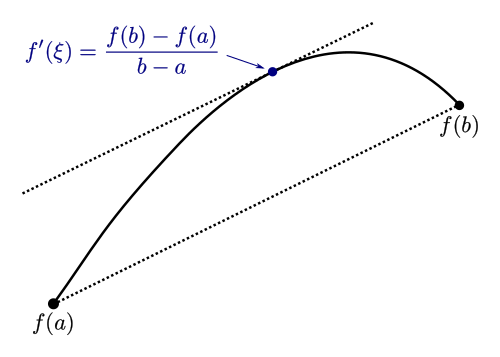
\includegraphics[width=0.6\textwidth]{images/Mittelwertsatz3.png}
      \caption{Quelle: Wikipedia}
\end{figure}
\begin{proof}
Setze $\gamma(t) := a + t(b-a), \; t \in [0,1]$ (Verbindungsgerade zwischen $a$ und $b$) und $F : = f  \circ \gamma : [0,1] \to \mathbb{R}$.
Damit ist $F(1)- F(0) = f(1) - f(0)$ und nach der Kettenregel ist $F$ differenzierbar.  Mit dem Mittelwertsatz einer Veränderlichen gibt es $\tau \in (0,1)$ mit 
$F(1) - F(0) = F'(\tau) = df(\gamma (\tau)) (b-a)$. Somit ist $\xi := \gamma(\tau)$ der gesuchte Punkt.
\end{proof}


\begin{Satz}[Satz von Schwarz]
Wenn Für eine Funktion $f: U \to \mathbb{R}$ die Ableitungen $\frac{\partial}{\partial x_i} f(a)$, $\frac{\partial}{\partial x_j}f(a)$ und $ \frac{\partial}{\partial x_i}\frac{\partial }{\partial x_j} f(a)$ existieren und letztere stetig ist, dann existiert auch $ \frac{\partial}{\partial x_j}\frac{\partial }{\partial x_i} f(a)$ und es gilt
\begin{align*}
\frac{\partial}{\partial x_i}\frac{\partial }{\partial x_j} f(a) = \frac{\partial}{\partial x_j}\frac{\partial }{\partial x_i} f(a)
\end{align*}
\end{Satz}

\fbox{\parbox{\linewidth}{
$\star \star \bigstar $  Bei wiederholten Ableiten spielt die Reihenfolge keine Rolle, wenn eine der Ableitungen existiert und stetig ist.
}}

\fbox{\parbox{\linewidth}{
$\diamond \Diamond $  Der Beweis geht in zwei Schritten: Man wendet den Mittelwertsatz einer Veränderlichen auf eine Hilfsfunktion an. Damit kann man die Differenz der Ableitungen abschätzen und zeigen, dass sie beliebig klein wird und damit gleich sind.
}}

\begin{proof}
Setze $\varphi(x,y) := f(a + x e_i + y e_j)$ mit $(x,y) \in  V \subset \mathbb{R}^2$. Bei hinreichend kleiner Wahl von $V$ existieren die Ableitungen $ \frac{\partial}{\partial y} \varphi$, $ \frac{\partial}{\partial x} \varphi$ und $ \frac{\partial}{\partial y} \frac{\partial}{\partial x} \varphi$  existiert und ist stetig nach Voraussetzung an $f$. Es reicht nun zu zeigen, dass $ \frac{\partial}{\partial x} \frac{\partial}{\partial y} \varphi (0,0)$ existiert  und 
\begin{align*}
\frac{\partial}{\partial x} \frac{\partial}{\partial y} \varphi(0,0) = \frac{\partial}{\partial y} \frac{\partial}{\partial x} \varphi (0,0)
\end{align*} 
gilt.  Sei dazu $\epsilon > 0$ und $V' \subset V$ so gewählt, dass $| \frac{\partial}{\partial y} \frac{\partial}{\partial x} \varphi(x,y) -  \frac{\partial}{\partial y} \frac{\partial}{\partial x} \varphi(0,0) | < \epsilon$ gilt für $(x,y) \in V'$.
Innerhalb eines achsenparallelen Quaders $Q \subset V'$  mit Ecken $(0,0)$ und $(h,k)$ setzen wir $u(x) := \varphi(x,  k) - \varphi(x, 0)$. Zweimaliges Anwenden des Mittelwertsatzes einer Veränderlichen liefert  
\begin{align*}
& u(h) - u(0) = hu'(\xi) \\
& = h(  \frac{\partial}{\partial x} \varphi(\xi, k) - \frac{\partial}{\partial x} \varphi(\xi, 0) ) = h k \frac{\partial}{\partial y} \frac{\partial}{\partial x} \varphi(\xi, \eta) \; .
\end{align*}
Damit erhalten wir die Abschätzung 
\begin{align*}
\biggl | \frac{ u(h) - u(0)}{hk} -   \frac{\partial}{\partial y} \frac{\partial}{\partial x} \varphi (0,0) \biggr | < \epsilon \; .
\end{align*}
Da 
\begin{align*}
& \lim_{k \to 0 } \frac{ u(h) - u(0)}{hk} =  \lim_{k \to 0 } \frac{1}{h} \biggl(   \frac{\varphi(h,k) - \varphi(h,0)  }{k}  -\frac{\varphi(0,k) - \varphi(0,0)  }{k} \biggr) \\
& =   \biggl(   \frac{  \frac{\partial}{\partial y} \varphi(h,0) -   \frac{\partial}{\partial y}\varphi(0,0)  }{k} \biggr) 
\end{align*}
und 
\begin{align*}
& \lim_{h \to 0 } \biggl(   \frac{  \frac{\partial}{\partial y} \varphi(h,0) -   \frac{\partial}{\partial y}\varphi(0,0)  }{k} \biggr) 
 =     \frac{\partial}{\partial x} \frac{\partial}{\partial y} \varphi(0,0) 
\end{align*}
folgt die Behauptung.
\end{proof}

\subsubsection*{Anwendung: Taylorreihe} 


\begin{Definition}[ $\mathcal{C}^k$-Funktion]
Eine  Funktion  $f: U \to \mathbb{R}$ für die alle partiellen Ableitungen 
\begin{align*}
 \frac{\partial}{\partial x_{i_1}} \cdots   \frac{\partial}{\partial x_{i_k}} f(a)
\end{align*}
mit $i_1 + \cdots + i_k \leq k$ existieren und stetig sind heißt $\mathcal{C}^k$-Funktion oder $k$-mal stetig differenzierbar. Eine 
$\mathcal{C}^1$-Funktion ist also eine differenzierbare Funktion.
\end{Definition}

\begin{Definition}[Höhere Ableitungen]
Für  eine Funktion  $f: U \to \mathbb{R}$, $a \in U$ und Vektoren $v^1, \cdots , v^p \in \mathbb{R}^n$ heißt 
\begin{align*}
d^pf(a) \bigl(v^1, \cdots , v^p  ) := \partial_{v^1} \hdots \partial_{v^p} f(a)
\end{align*}
die $p$-te Richtungsableitung von $f$. Sie ist wegen dem Satz von Schwarz wohldefiniert.
Mit Bemerkung \ref{partial1} ist
\begin{align*}
d^pf(a) \bigl(v^1, \cdots , v^p  ) = \sum_{i_1 = 1}^n \cdots \sum_{i_p = 1}^n  \frac{\partial}{\partial x_{i_1}} \hdots \frac{\partial}{\partial x_{i_p}} f(a) \cdot v^1_{i_1} \cdots v^p_{i_p} \; .
\end{align*}
Für einen Vektor $z \in \mathbb{R}^n$ definieren wir $$d^pf(a) z^p := d^pf(a) \underbrace{(z, \cdots , z)}_{p-mal} \;.$$

\end{Definition}



\begin{Bemerkung}
Für $p = 2$ und $u,v \in \mathbb{R}^n$ ist
\begin{align*}
d^2f(a) \bigl(u , v ) = \sum_{i = 1}^n \sum_{j = 1}^n \frac{\partial}{\partial x_{i}}  \frac{\partial}{\partial x_{j}} f(a) v_{i}  u_{j} 
\end{align*}
und mit 
\begin{align*}
f''(a) : = \begin{pmatrix}  \frac{\partial}{\partial x_{1}} \frac{\partial}{\partial x_{1}} f(a)   &  \cdots &  \frac{\partial}{\partial x_{1}} \frac{\partial}{\partial x_{n}} f(a) \\
\vdots & & \vdots  \\
 \frac{\partial}{\partial x_{n}} \frac{\partial}{\partial x_{1}} f(a)   &  \cdots &  \frac{\partial}{\partial x_{n}} \frac{\partial}{\partial x_{n}} f(a)
\end{pmatrix} 
\end{align*}
ist $d^2f(a) \bigl(u , v ) = u^T  \cdot f''(a) \cdot v$. Die Matrix $f''(a)$ wird auch Hesse-Matrix genannt. Nach dem Satz von Schwarz ist sie symmetrisch.
\end{Bemerkung}


\begin{Satz}[Taylorapproximation]
Sei   $f: U \to \mathbb{R}$ eine $\mathcal{C}^{p+1}$-Funktion und $x,a \in U$, so dass die Verbindung zwischen $x$ und $a$ in $U$ liegt.
Dann gilt
\begin{align*}
f(x) = f(a) + \sum_{k=1}^{p} d^k f(a) (x-a)^k + R_{p+1} (x,a)
\end{align*}
mit dem Restglied $R_{p+1} (x,a) := \frac{1}{(p+1)!} d^{p+1}f(\xi) (x-a)^{p+1}$ für ein $\xi \in [a,x]$.
\end{Satz}

\begin{proof}
Sei $h := (x-a)$ und $F(t) := f(a + th)$ mit $t \in [0,1]$. Wiederholte Anwendung der (Baby) Kettenregel mit $\gamma(t) := a +th$ ergibt
\begin{align*}
& F'(t) = \sum_{i=1}^n  \frac{\partial}{\partial x_{i}} f(a + th) h_i \\
& F''(t) =\sum_{j=1}^n \sum_{i=1}^n   \frac{\partial}{\partial x_{j}} \frac{\partial}{\partial x_{i}} f(a + th) h_i h_j \\
& \vdots \\
& F^p(t) =  \sum_{i_1=1}^n  \cdots \sum_{i_p=1}^n   \frac{\partial}{\partial x_{i_1}} \cdots \frac{\partial}{\partial x_{i_p}} f(a + th) h_{i_1} \cdots  h_{i_p}  \; .
\end{align*}
Mit der Taylorapproximation für Funktionen einer Veränderlichen folgt
\begin{align*}
 F(1) = F(0) + F'(0) + \frac{1}{2!} F''(0) + \cdots + \frac{1}{p!} F^p(0) + R_{p+1} 
\end{align*}
mit dem Restglied $ R_{p+1}  :=  \frac{1}{(p+1)!}  F^p(\tau)$ mit $\tau \in [0,1]$.
Da nach Konstruktion $F(0) = f(a)$ und $F(1)= f(x)$ folgt insgesamt die Behauptung.
\end{proof}


\begin{Satz}[Qualitative Taylorformel]
Sei $T_p(x,a) =  f(a) + \sum_{k=1}^{p} d^k f(a) (x-a)^k$ die Taylorraproximation einer $\mathcal{C}^{p}$-Funktion. Dann gilt: 
\begin{align*}
\lim_{x \to a} \frac{f(x) - T_p(x,a)}{  || x-a  ||^p} = 0 \;. 
\end{align*}
\end{Satz}
\begin{proof}
Da die partiellen Ableitungen stetig sind, gibt es für jedes $\epsilon > 0$ ein Radius $r >0$, dass für alle $y \in K_r(a)$
\begin{align*}
\frac{1}{p!} (d^pf(y) -d^pf(a))h^p \leq \epsilon ||h||_{\infty}^p \; . 
\end{align*}
Mit der Taylorapproximation ist 
\begin{align*}
f(x) = T_{p-1}(x, a) +  \frac{1}{p!} d^{p}f(\xi) (x-a)^{p} = T_p(x,a) +  \frac{1}{p!} \bigl( d^pf(\xi) -d^pf(a) \bigr) h^p (x-a)^p
\end{align*} 
Mit obiger Abschätzung folgt die Behauptung.
\end{proof}

\subsection{Extrema}

\begin{Definition}[Extremum]
Sei $f : X \subset \mathbb{R}^n \to \mathbb{R}$ eine relle Funktion.  Ein Punkt $a \in  X$ heißt lokales Maximum bzw. Minimum, falls eine Umgebung $U$ von $a$ existiert, so dass $f(x) \leq f(a)$ bzw.  $f(x) \geq f(a)$ für alle $x \in U$ gilt. Liegt einer der beiden Fälle vor, so spricht man von einem lokalen Extremum. Gilt strikt $f(x) <  f(a)$ bzw.  $f(x) > f(a)$ , so nennt man das Extremum isoliert. Ist $U = X$ so nennt man es auch globales Maximum bzw. Minimum.
\end{Definition}


\begin{figure}[H]
      \centering
    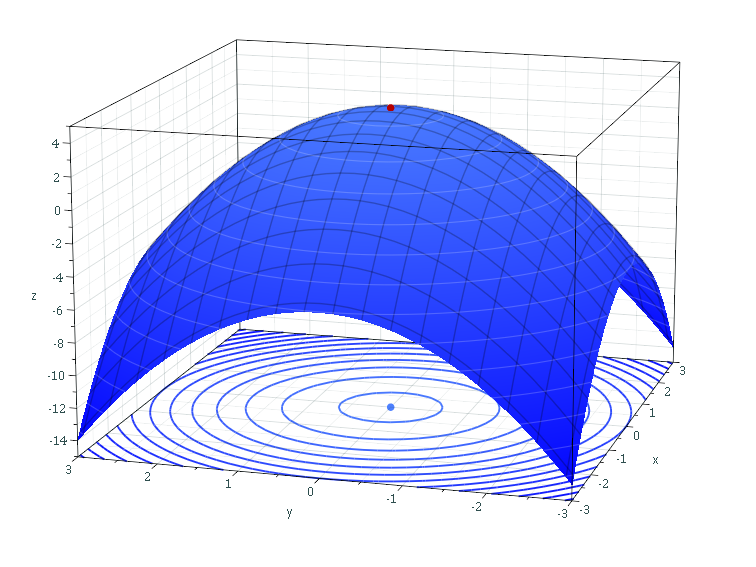
\includegraphics[width=0.6\textwidth]{images/MaximumParaboloid}
      \caption{Quelle: Wikipedia: https://en.wikipedia.org/wiki/File:MaximumParaboloid.png}
    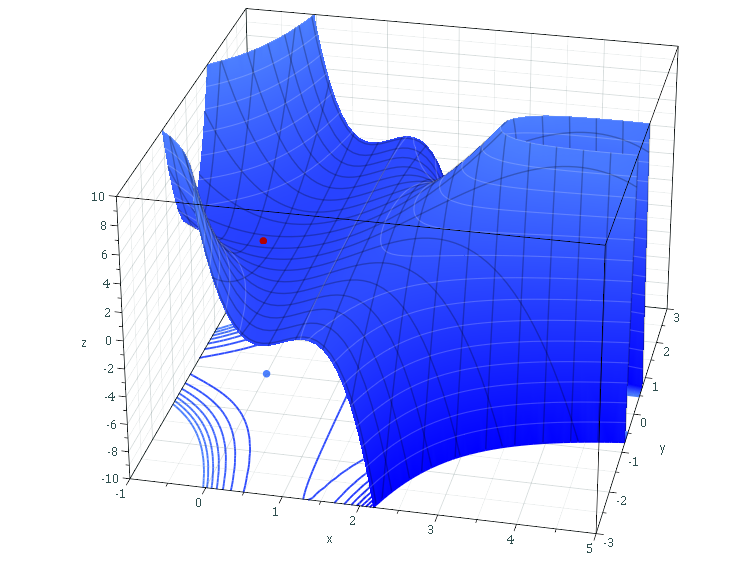
\includegraphics[width=0.6\textwidth]{images/MaximumCounterexample}
      \caption{Quelle: Wikipedia: https://en.wikipedia.org/wiki/File:MaximumCounterexample.png}
\end{figure}


\begin{Satz}[Notwendiges Kriterium]
 Ist $f: U  \to \mathbb{R}$ differenzierbar und hat  $f$ in $a \in U$ ein lokales Extremum, so gilt 
\begin{align*}
\frac{\partial}{\partial x_{1}}f(a)  = \cdots  = \frac{\partial}{\partial x_{n}} f(a) = 0 \;.
\end{align*}
Dies ist gleichbedeutend mit $df(a) = 0$.
\end{Satz}
\begin{proof}
Setze $F_k(t) := f(a + t e_k)$. Da $f$ ein Extremum in $a$ hat, hat $F_k$ in einer hinreichend kleinen Umgebung um $0$ ein Extremum. 
Da $F_k$ eine Funktion einer Veränderlichen ist, gilt $F'(0) = 0$. Da $\frac{\partial}{\partial x_k} f(a) = F_k'(0)$ folgt die Behauptung.
\end{proof}

\begin{Definition}[Kritischer Punkt]
Ein Punkt $a$ mit $df(a) = 0$ wird als kritischer Punkt Bezeichnet. 
\end{Definition}

\begin{Satz}[Hinreichendes Kriterium]
 Ist $f: U  \to \mathbb{R}$ eine $\mathcal{C}^2$-Funktion und ist $f'(a) = 0$  ein kritischer Punkt für ein $a \in U$. Dann gilt:
\begin{itemize}
\item $f''(a) > 0 \Rightarrow $ $f$ hat in $a$ ein isoliertes lokales Minimum.
\item $f''(a) < 0 \Rightarrow $ $f$ hat in $a$ ein isoliertes lokales Maximum.
\item $f''(a) \gtrless 0 \Rightarrow $ $f$ hat in $a$ einen Sattelpunkt.
\end{itemize} 
\end{Satz}
\begin{proof}
Sei $f'(a) = 0$ und $f''(a) > 0$. Mit der Taylorformel gilt für hinreichend kurze Vektoren $h \in \mathbb{R}^n$
\begin{align*}
f(a + h) = f(a) + \frac{1}{2} h^T f''(a) h + R(h)
\end{align*}
mit $\lim_{h \to 0} \frac{R(h)}{ ||h||^2} = 0$. Für $||h|| \leq 1$ hat $ h^T f''(a) h $ sein Maximum $m$ auf dem Einheitskreis $\{ h \in \mathbb{R}^n \; | \; ||h|| = 1 \}$ da $f''(a) > 0$.
\begin{align*}
 h^T f''(a) h  = ||h|| \frac{1}{||h||} h^t  f''(a)  ||h|| \frac{1}{||h||} h \geq m ||h||^2 \;.
\end{align*}
Wir wählen $\epsilon$ so klein, dass $R(h) \leq \frac{m}{2}  ||h||^2$ gilt für $||h|| < \epsilon$  (was geht wegen Taylorformel).
Damit erhalten wir
\begin{align*}
f(a + h) \geq f(a) +  m ||h||^2 \;.
\end{align*}
und damit hat $f$ ein lokales Minimum in $a$.

Der Fall $f''(a) < 0$ wird mit Betrachtung von $-f$ durch den vorigen Fall bewiesen.

Es sei nun $f''(a) \gtrless 0$ und $v$ mit $v^T f''(a) v > 0$ und $w$ mit $w^T f''(a) w > 0$. Betrachten wir die Funktionen
\begin{align*}
F_v (t) := f(a + tv) \\
F_w(t) := f(a +tw)
\end{align*}
dann ist 
\begin{align*}
F_v' (t) = 0; \; F_v''(0) = v^T f''(a) v > 0 \\
F_w' (t) = 0; \; F_w''(0) = w^T f''(a) w < 0 \\
\end{align*}
und somit hat $F_v$ ein isoliertes lokales Maximum und $F_w$ ein isoliertes lokales Minimum und damit $f$ kein lokales Extremum  in  $a$.
\end{proof}


\begin{figure}[H]
      \centering
    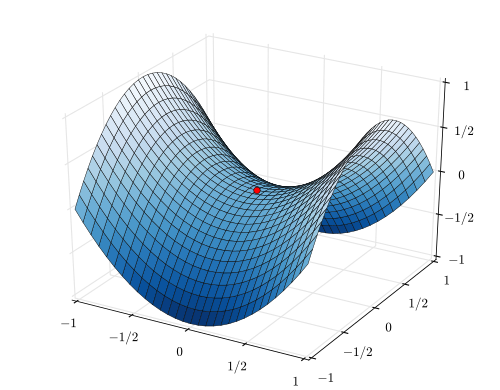
\includegraphics[width=0.6\textwidth]{images/Saddle_point}
      \caption{Quelle: Wikipedia: https://commons.wikimedia.org/wiki/File:Saddle\_point.svg}

\end{figure}



\subsubsection*{Anwendung: Gradientenverfahren} 
Wie kann man Minima einer  differenzierteren Abbildung $f: \mathbb{R}^n \to \mathbb{R}$ finden? 
Wir wissen, dass an jedem Punkt $x_k \in  \mathbb{R}^n$ der negative Gradient  $d_k := -\nabla f (x_k)$ in die steilste Abstiegsrichtung zeigt.
Die Idee des Gradientenabstieg ist, ein bestimmtes  Stück in diese Richtung abzusteigen, damit der Funktionswert kleiner wird, also $x_{k+1} = x_k + \alpha_k d_k$ zu setzen. Für hinreichend kleines $\alpha_k$ folgt mit Satz \ref{lokaleLinearisierung} über die lokale Liberalisierung  
$f(x_{k+1}) = f (x_k + \alpha_k d_k) =  f(x_k) + \alpha_k df(x_k)d_k + R( \alpha_k dk)$.  Somit gilt $f(x_{k+1}) \leq f(x_k)$, falls $\nabla f(x_k) \neq 0$ und falls die folge $f(x_k)$ beschränkt ist, so ist  dieser Fixpunkt $x^*$ ein minimum, da $\nabla f(x^*) = 0$ gelten muss.  

\begin{algorithm}
\caption{Gradienentabstieg}
\begin{algorithmic}[1]


    \State Initialisiere $k:=0$ und zufälligen Startwert $x_0$.
\State Initialisiere Genauigkeit $\epsilon > 0$.
    \While{$|| \nabla f(x_k) || > \epsilon$}  \Comment{So lange kein Extrema vorliegt}
        \State Bestimme $\alpha_k$  mit $f (x_k + \alpha d_k) =  f(x_k) + \alpha_k df(x_k)d_k + R( \alpha_k dk)$ \Comment{Schrittweite bestimmen}
        \State Setze $x_{k+1} := x_k  + \alpha_k d_k$. \Comment{Absteigen}
 	\State  $k \leftarrow k+1$ \Comment{Wiederholen}
    \EndWhile  \label{Gradientenverfahren}


\end{algorithmic}
\end{algorithm}

\begin{figure}[H]
      \centering
    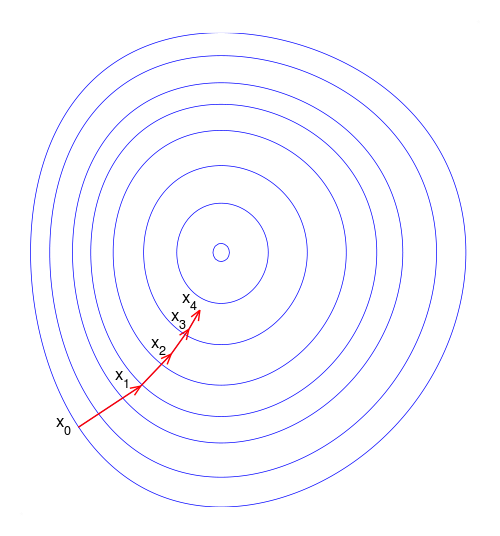
\includegraphics[width=0.7\textwidth]{images/Gradient_descent}
      \caption{Quelle: Wikipedia}
\end{figure}



\begin{Definition}
Sei  $f: \mathbb{R}^n \to \mathbb{R}$  eine differenzierbare Funktion. Eine Kurve $\gamma : I \to \mathbb{R}^n$, auf der $f$ konstant ist, also 
$f(\gamma(t)) = c$ für eine festes $c \in \mathbb{R}$ gilt, heißt Höhenlinie.
\end{Definition}

\begin{figure}[H]
      \centering
    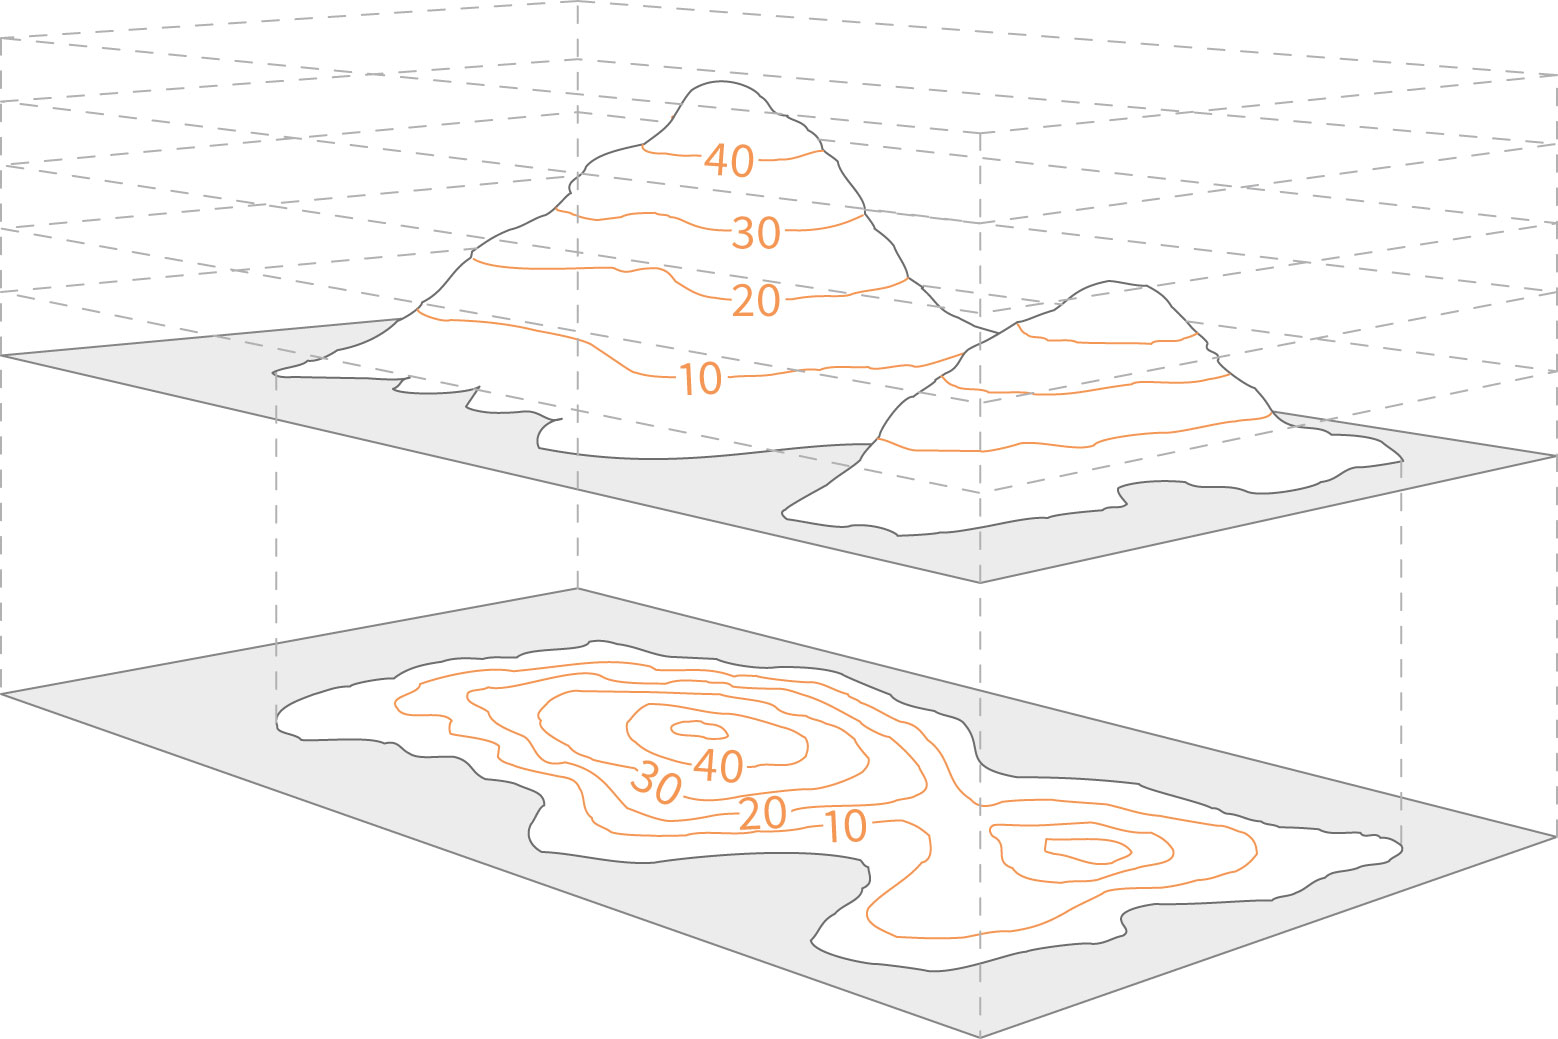
\includegraphics[width=0.8\textwidth]{images/Contours-and-relief}
      \caption{Quelle: https://getoutside.ordnancesurvey.co.uk/guides/understanding-map-contour-lines-for-beginners/}
\end{figure}


\begin{Bemerkung}
Der Gradient steht senkrecht auf  Höhenlinien. Dies bedeutet, dass $$ \bigl \langle \nabla f(\gamma(t)), \gamma'(t) \bigr \rangle = 0$$ gilt. 
\end{Bemerkung}
\begin{proof}
Aus $f(\gamma(t)) = c$ folgt $\frac{d}{dt} f(\gamma(t)) = 0$. Mit der Kettenregel folgt $\frac{d}{dt} f(\gamma(t)) =  f(\gamma(t)) \cdot \gamma'(t) = 0$ und damit
$ \bigl \langle \nabla f(\gamma(t)), \gamma'(t) \bigr \rangle = 0$.
\end{proof}

\subsubsection*{Anwendung: Backpropagation}
Ein Neuronales Netz ist eine Funktion $f : \Omega \times \mathbb{R}^n \to \mathbb{R}^m$, die einem Input (auch Feature genannt) in Abhängigkeit der Gewichte $\Omega$
einen Ausgabewert zuordnet. Die Funktion ist dabei aus einfachen Bausteinen zusammengesetzt.

\begin{figure}[H]
      \centering
    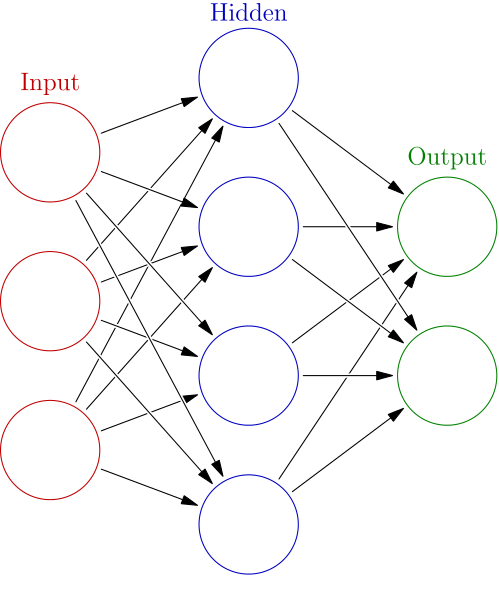
\includegraphics[width=0.4\textwidth]{images/499px-Colored_neural_network}
      \caption{Quelle: Wikipedia}
    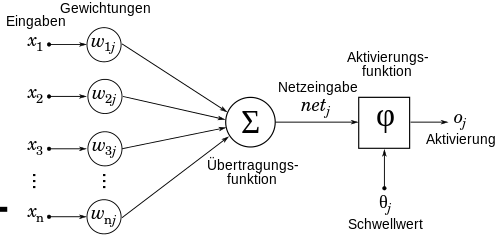
\includegraphics[width=0.6\textwidth]{images/500px-NeuronModel_deutsch}
      \caption{Quelle: Wikipedia}
\end{figure}


Gegeben ist ein  Datensatz $D : = \{ (x_i, y_i) \}$. Finde Gewichte Omega, so dass Lossfunktion
\begin{align*}
L_D  : \Omega \subset \mathbb{R}^n \to \mathbb{R} 
\end{align*}
minimal wird. Zum Beispiel $L_D(\omega) := \sum_{(x_i,y_i) \in D} (f(\omega, x_i) - y_i)^2$.

Wende Gradientenverfamren an:

\begin{algorithm}
\caption{Gradientabstieg}
\begin{algorithmic}[1]
    \State Initialisiere $k:=0$ und zufällige Gewichte $w_0$.
\State Initialisiere Genauigkeit $\epsilon > 0$.
    \While{$|| \nabla L_D(\omega) || > \epsilon$}  \Comment{So lange kein Extrema vorliegt}
        \State Bestimme $\alpha_k$  mit $ L_D(\omega_k + \alpha d_k) =  L_D(\omega_k) + \alpha_k d L_D(\omega_k)d_k + R( \alpha_k dk)$ \Comment{Schrittweite bestimmen}
        \State Setze $\omega_{k+1} := \omega_k  + \alpha_k d_k$. \Comment{Absteigen}
 	\State  $k \leftarrow k+1$ \Comment{Wiederholen}
    \EndWhile  \label{roy's loop}


\end{algorithmic}
\end{algorithm}

Wenn der Datensatz $D$ sehr groß ist (Big Data), ist die Berechnung des Gradient der Lossfunktion entsprechend aufwendig. Um diesen Aufwand zu reduzieren,
kann man das Gradientenverfamren modifizieren, so dass man Gradienten nur auf Teilräumen berechnet. Man erhält somit das sogenannte Mini-Batch Gradientenverfamren und das stochastische Gradientenverfamren.

\begin{algorithm}
\caption{Gradientabstieg}
\begin{algorithmic}[1]
    \State Initialisiere $k:=0$ und zufällige Gewichte $w_0$.
\State Initialisiere Genauigkeit $\epsilon > 0$.
\State Wähle Teilmenge $D_0' \subset D$
    \While{$|| \nabla L_{D'_k}(\omega) || > \epsilon$}  \Comment{So lange kein Extrema vorliegt}
        \State Bestimme $\alpha_k$  mit $ L_{D'_k}(\omega_k + \alpha d_k) =  L_{D'_k}(\omega_k) + \alpha_k d L_{D'_k}(\omega_k)d_k + R( \alpha_k dk)$ \Comment{Schrittweite bestimmen}
        \State Setze $\omega_{k+1} := \omega_k  + \alpha_k d_k$. \Comment{Absteigen}
	\State Wähle neue Teilmenge $D'_{k +1} \subset D$.
 	\State  $k \leftarrow k+1$ \Comment{Wiederholen}
    \EndWhile  \label{roy's loop}


\end{algorithmic}
\end{algorithm}

Wenn man als Teilmenge immer nur eine einelementige Menge wählt, so spricht man vom stochastischen Gradientenverfahren.

\begin{figure}[H]
      \centering
    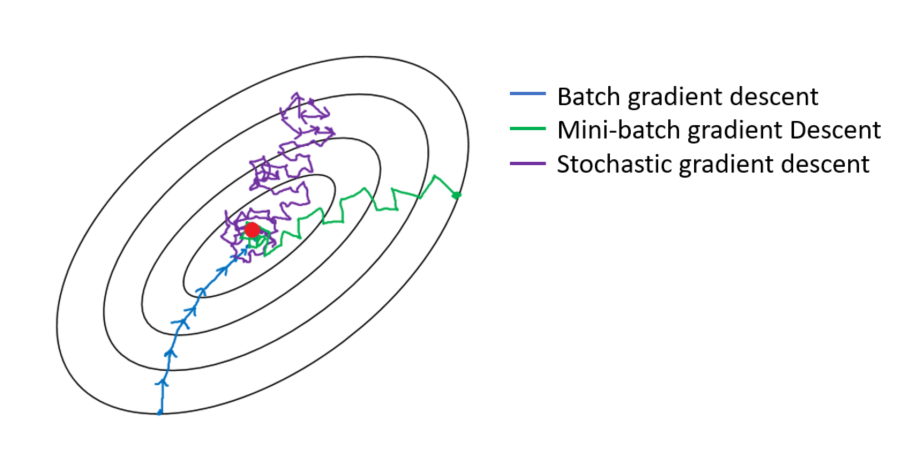
\includegraphics[width=1.0\textwidth]{images/batchgradient}
      \caption{Quelle: https://towardsdatascience.com/batch-mini-batch-stochastic-gradient-descent-7a62ecba642a}
\end{figure}


\subsection{Gradient einer  mehrdimensionalen Funktion}
\begin{Definition}
\label{diffbarkeitmd}
Eine Funktion $F: U \to \mathbb{R}^m$ heißt differenzierbar, wenn es eine lineare Abbildung $dF$ gibt, so dass 
\begin{align*}
F(a + h) = F(a) + dF(a)h + R(h)
\end{align*}
mit $\lim_{h \to 0} \frac{R(h)}{||h||} = 0$ gilt für alle $a \in U$ und $h \in \mathbb{R}^n$.
\end{Definition}

\begin{Bemerkung}
Im Fall $n = 1$ stimmt diese Definition mit der alten Definition \ref{diffbarkeit} überein.
\end{Bemerkung}
\begin{proof}
Nach Satz \label{lokaleLinearisierung} gilt für eine differenzierbare Funktion $f(a + th) = f(a) + df th + R(th)$ mit  $\lim{t \to 0} \frac{R(th)}{||th||} = 0$. Umstellen ergibt
\begin{align*}
df(a) h = \lim_{t \to 0} \frac{f(a + th) - f(a)}{t}
\end{align*} 
und somit existieren alle linearen Abbildungen und wegen der Linearität von $df$ sind diese auch stetig.
\end{proof}

\begin{Beispiel}[Affine Abbildung]
Für $A \in \mathbb{R}^{n \times n}$, $b \in \mathbb{R}^n$  ist die Abbildung $F(x) := Ax +b$ differenzierbar, da
$F(a +h) = A(a+h) + b = A a+ Ah +b = Aa +b + Ah = F(a) + Ah$ und damit für $dF(a) := A$ und $R(h) = 0$ die Definition \ref{diffbarkeitmd}
 erfüllt ist.
\end{Beispiel}

\begin{Satz}[Differenzierbarkeit von Produktfunktionen]
Eine Funktion $F:= (F_1, F_2) : U  \to \mathbb{R}^m \times \mathbb{R}^k$ ist genau dann differenzierbar, 
wenn $F_1 : U  \to \mathbb{R}^m$ und   $F_2 : U  \to \mathbb{R}^k$ differenzierbar sind. In diesem Fall ist
$$dF(a) = (dF_1(a), df_2 (a)) \;.$$ 
\end{Satz}
\begin{proof}
Sind $F_1$ und $F_2$ differenzierbar, so gilt für $i = 1,2$
\begin{align*}
F_i (a + h) = F_i(a) + dF_ih + R_i(h)
\end{align*}
Dann gilt mit $dF(a) = (dF_1(a), df_2 (a))$ und $R(h):= (R_1(h), R_2(h))$
\begin{align*}
F (a + h) = F (a) + dF h + R(h)
\end{align*}
mit $\lim_{h \to 0} \frac{R(h):}{||h||} = 0$ und damit ist $F$ differenzierbar. Die Umkehrung folgt analog.
\end{proof}

\begin{Bemerkung}[Differenzial von  Produkfunktionen]
Eine Abbildung $F : U \to \mathbb{R}^m$ ist genau dann  differenzierbar, wenn ihre Koordinaten-Funktionen 
$F_1 : U \to \mathbb{R},  \cdots, F_m : U \to \mathbb{R}$ mit $F(a) = \begin{pmatrix} F_1(a) \\ \vdots \\ F_m(a) \end{pmatrix}$ differenzierbar sind. In diesem Fall gilt
\begin{align*}
dF(a) :=   \begin{pmatrix}  \frac{\partial}{\partial x_1}  F_1(a) & \cdots & \frac{\partial}{\partial x_n} F_1(a) \\ 
\vdots & & \vdots \\
\frac{\partial}{\partial x_1}  F_m(a) & \cdots & \frac{\partial}{\partial x_n} F_m(a) 
\end{pmatrix}
\end{align*}
\end{Bemerkung}

\begin{Bemerkung}[Differenzierbarkeit von Wegen]
Ein Weg $\gamma =  \begin{pmatrix} \gamma_1  \\ \vdots \\ \gamma_m \end{pmatrix} : I \to U$ ist genau dann differenzierbar, wenn $\gamma_i$ differenzierbar ist für $i= 1, \cdots, m$ und dann gilt $\gamma'(t) =   \begin{pmatrix} \gamma'_1(t)  \\ \vdots \\ \gamma'_m(t) \end{pmatrix} \; .$
\end{Bemerkung}



\begin{Satz}[Kettenregel]
Seien $G:  U \subset \mathbb{R}^n \to V \subset \mathbb{R}^m$ und $F: V \to Z \subset \mathbb{R}^k$ differenzierbar. Dann ist $F \circ G$ differenzierbar und mit $b := G(a)$ es gilt
$$ d(F \circ G)(a) = dF(b) \cdot dG(a) $$
\end{Satz}
\begin{proof}
Analog zu Baby Kettenregel.
\end{proof}


\subsubsection*{Anwendung: Automatisches Ableiten} 


\begin{figure}[H]
      \centering
    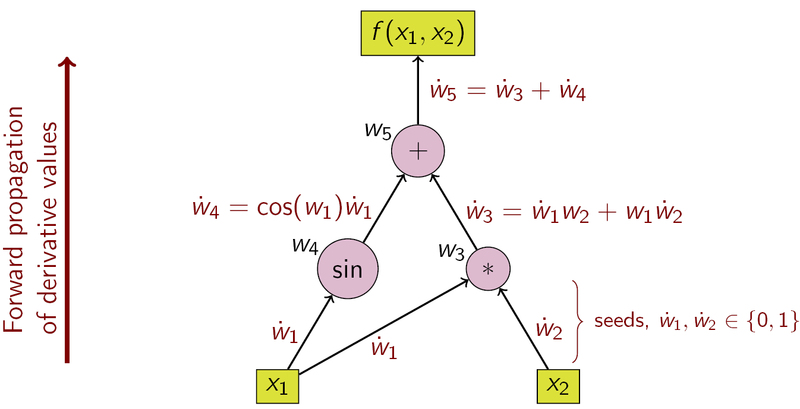
\includegraphics[width=0.8\textwidth]{images/ad.png}
      \caption{Quelle: Wikipedia}
\end{figure}

\href{https://pytorch.org/tutorials/beginner/blitz/autograd_tutorial.html}{Automatisches Ableiten  in Pytorch}

Mit Hilfe des Automatischen Ableiten kann man den Gradienten der Lossfunktion zu einem Neuroyalen Netzt einfach berechnen, da dieser sich aus einfachen Funktionen zusammensetzt.








\section{Mehrdimensionale Integralrechnung}

\subsection{Lebesgue Maß}

Für offene Intervalle $(a_i,b_i) \subset \mathbb{R}$ mit $a_i \leq b_i$ nennen wir $I := (a_1,b_1) \times \cdots \times (a_n,b_n)$ einen $n$-dimensionalen Quader 
und $\bar{I}:= [a_1, b_1] \times \cdots \times [a_n,b_n]$ seinen Abschluss. Wir definieren das Volumen 
\begin{align*}
\text{vol} (I):=   \prod_{i = 1}^n (b_i -a_i)  \; .
\end{align*}

Mit 
$$\mathbb{I}(n): = \{   (a_1,b_1) \times \cdots \times (a_n,b_n) \; | \;  (a_i, b_i) \subset \mathbb{R} \}$$
 bezeichnen wir die Menge aller $n$-dimensionalen Quader und mit
$$\mathbb{I}^0(n): = \{   (a_1,b_1) \times \cdots \times (a_n,b_n) \; | \;  (a_i, b_i) \subset \mathbb{R}  \text { und } a_k = b_k \text{ für ein k}\}$$ 
die Menge der degenerierten Quader.   Für eine Menge $A \subset \mathbb{R}^n$ bezeichnen wir eine Menge von Quadern 
$$ \biggl \{ I_j \; | \;  I_j \in \mathbb{I}(n)   \text{ mit } A \subset \bigcup_j I_j  \biggr \}$$ als Hüllquader für $A$.
\begin{Definition}[Lebesguesche äußere Maß]
Für eine Menge $A \subset \mathbb{R}^n$ definieren wir das Lebesguesche äußere Maß durch 
\begin{align*}
\mu (A):=   \inf \biggl \{ \sum_{j=1}^{\infty}   \text{vol} (I_j)\; ; \; I_j \in \mathbb{I}(n); A \subset \bigcup_{j= 1}^{\infty} I_j \biggr \} 
\end{align*}
Falls für alle Hüllquader $\text{vol} (I_j) = \infty$ gilt, so setzen wir $\mu (A) = \infty$.
\end{Definition}

\begin{Definition}[Erinnerung Infimum]
\end{Definition}

\begin{Definition}[Nullmenge]
Eine Menge $N \subset \mathbb{R}^n$ mit $\mu (N) = 0$ heißt Nullmenge.
\end{Definition}


\begin{Bemerkung}
\label{massmonton}
Für $A \subset B \subset \mathbb{R}^n$ ist $\mu(A) \leq \mu(B)$
\end{Bemerkung}
\begin{proof}
Da $A \subset B$ Teilmenge ist, sind Hüllquader von $B$  auch Hüllquader von $A$ und damit  $\mu(A) \leq \mu(B)$.
\end{proof}

\begin{Satz}[$\sigma$-subadditivität]
Sei $A_j \subset \mathbb{R}^n$ eine Folge von Mengen. Dann gilt
\begin{align*}
\mu (\bigcup_j^{\infty} A_j ) \leq \sum_{j=1}^{\infty} \mu(A_j)
\end{align*}
\end{Satz}
\begin{proof}
Für jedes $A_j$ und $\epsilon > 0$ können wir  eine geeignete Überdeckung  $A_j \subset \bigcup_k  K_{j,k}$ mit Hüllquadern $K_{j,k}$ finden, so dass 
 $\sum_k \text{vol} (K_{j,k}) \leq \mu(A_j) + \frac{\epsilon}{2^{j+1}}$.
Da $ \bigcup_j A_j \subset \bigcup_j \bigcup_k  K_{j,k}$ eine Überdeckung mit Hüllquadern ist, folgt
\begin{align*}
\mu \biggl (  \bigcup A_j  \biggr) \leq \sum_j \sum_k \text{vol} (K_{j,k}) \leq  \bigl( \sum_j  \mu(A_j) + \frac{\epsilon}{2^{j+1}} \bigr)  = \bigl (\sum_j \mu(A_j) \bigr ) + \epsilon
\end{align*}
(Die letzte Gleichung beruht auf dem Wert der \href{https://de.wikipedia.org/wiki/Geometrische_Reihe}{geometrischen Reihe}).
Da die letzte Aussage für beliebiges $\epsilon > 0$ gilt, folgt die Behauptung.
\end{proof}


\begin{Bemerkung}
\label{volimu}
Für $I \in \mathbb{I}(n)$ gilt $\mu(I) = \text{vol}(I)$.
\end{Bemerkung}
\begin{proof}
Seien  $I_j \in \mathbb{I}(n)$ mit $I \subset \bigcup_j  I_j$. Da $I$ beschränkt und abgeschlossen ist, ist $I$ kompakt. Damit reichen endlich 
viele Intervalle, um $I  \subset  \bigcup_{j=1}^n  I_j$ zu überdecken. Für endlich viele Intervalle ist es einfach zu zeigen, dass
$$\text{vol} (I) \leq \sum_{j=1}^n \text{vol} (I_j) $$
gilt. Damit folgt die Behauptung.
\end{proof}

\begin{Satz}
Für $I \in \mathbb{I}(n)$  und $A \subset \mathbb{R}^n$ mit $I \subset A \subset \bar{I}$ gilt $\mu (A) = \text{vol}(I)$.
\end{Satz}
\begin{proof}
Mit $I_0:=  I$ und $I_j := \emptyset$ ist $I \subset \bigcup_j I_j$ und damit gilt 
\begin{align*}
\mu(I) \leq \sum_j \text{vol}(I_j) = \text{vol}(I)
\end{align*}

Es sei $\mathcal{A}_0 := \{ A  \in \mathbb{R}^n  \; | \;  I^0 \subset A \subset \bar{I^0}  \text{  mit } I^0 \in \mathbb{I}^0(n) \}$. Für $A_0 \in \mathcal{A}_0$ gibt es 
$\epsilon > 0$ und $I_{\epsilon} \in \mathbb{I}(n)$ mit $A \subset I_{\epsilon}$ und $\text{vol} (I_{\epsilon})  \leq \epsilon$ und damit $\mu(A_0) = 0$.
Zu $I \in \mathbb{I}(n)$ gibt es $2n$-Seiten $J_j \in \mathcal{A}_0$ mit 
$\bar{I} = I \cup \bigcup_{j= 1}^{2n} J_j$. Aus der $\sigma$-subadditivität folgt
\begin{align*}
\mu(\bar{I})  \leq \mu(I) + \sum_{j=1}^{2n} \mu(J_j) = \mu (I)
\end{align*}
 Für $I \subset A \subset \bar{I}$ folgt damit und mit der Monotonie
$$ \mu(I) = \mu(A) = \mu(\bar{I}) \;. $$
Mit Bemerkung \ref{volimu} folgt die Behauptung.

\end{proof}


Es sei $A, D \subset \mathbb{R}^n$  beschränkte Teilmenge mit $A \subset D$.  
Man kann einerseits das Volumen $\mu(A)$, als auch das Volumen 
$\mu_D(A) :=  \mu(D) - \mu(D  \setminus  A)$ berechnen. Man approximiert hierbei das Volumen von $A$ einmal mit Hüllquadern von außen und einmal von innen.
 
\begin{figure}[!tbp]
  \centering
  \begin{minipage}[b]{0.49\textwidth}
    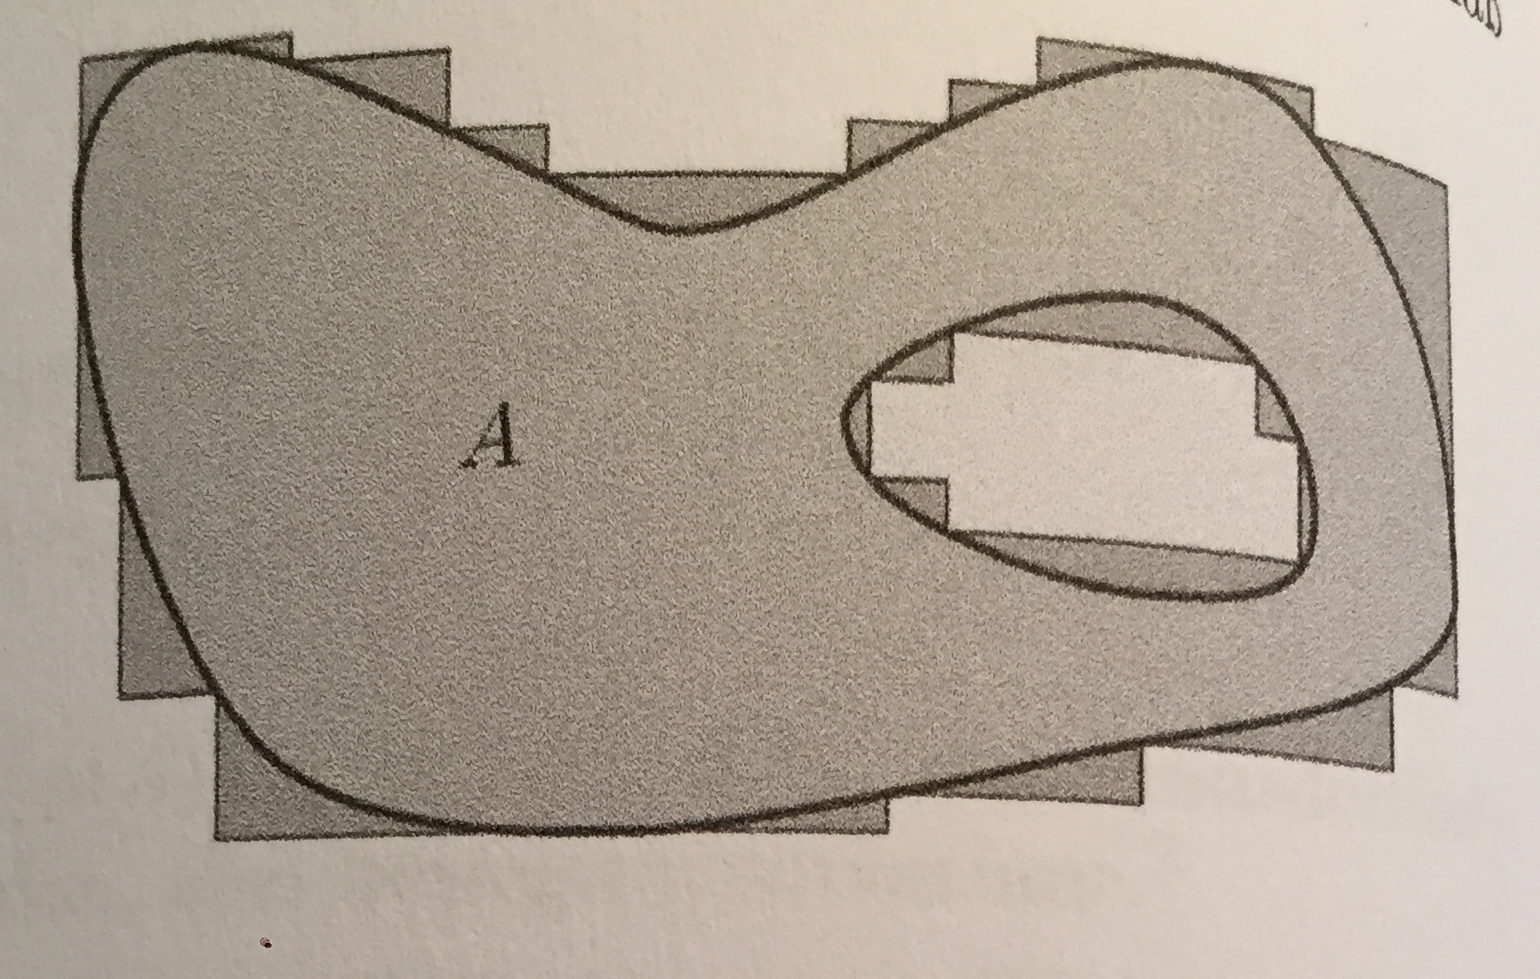
\includegraphics[width=1.0\textwidth]{images/am}
    \caption{Äußeres Maß}
  \end{minipage}
  \hfill
  \begin{minipage}[b]{0.49\textwidth}
    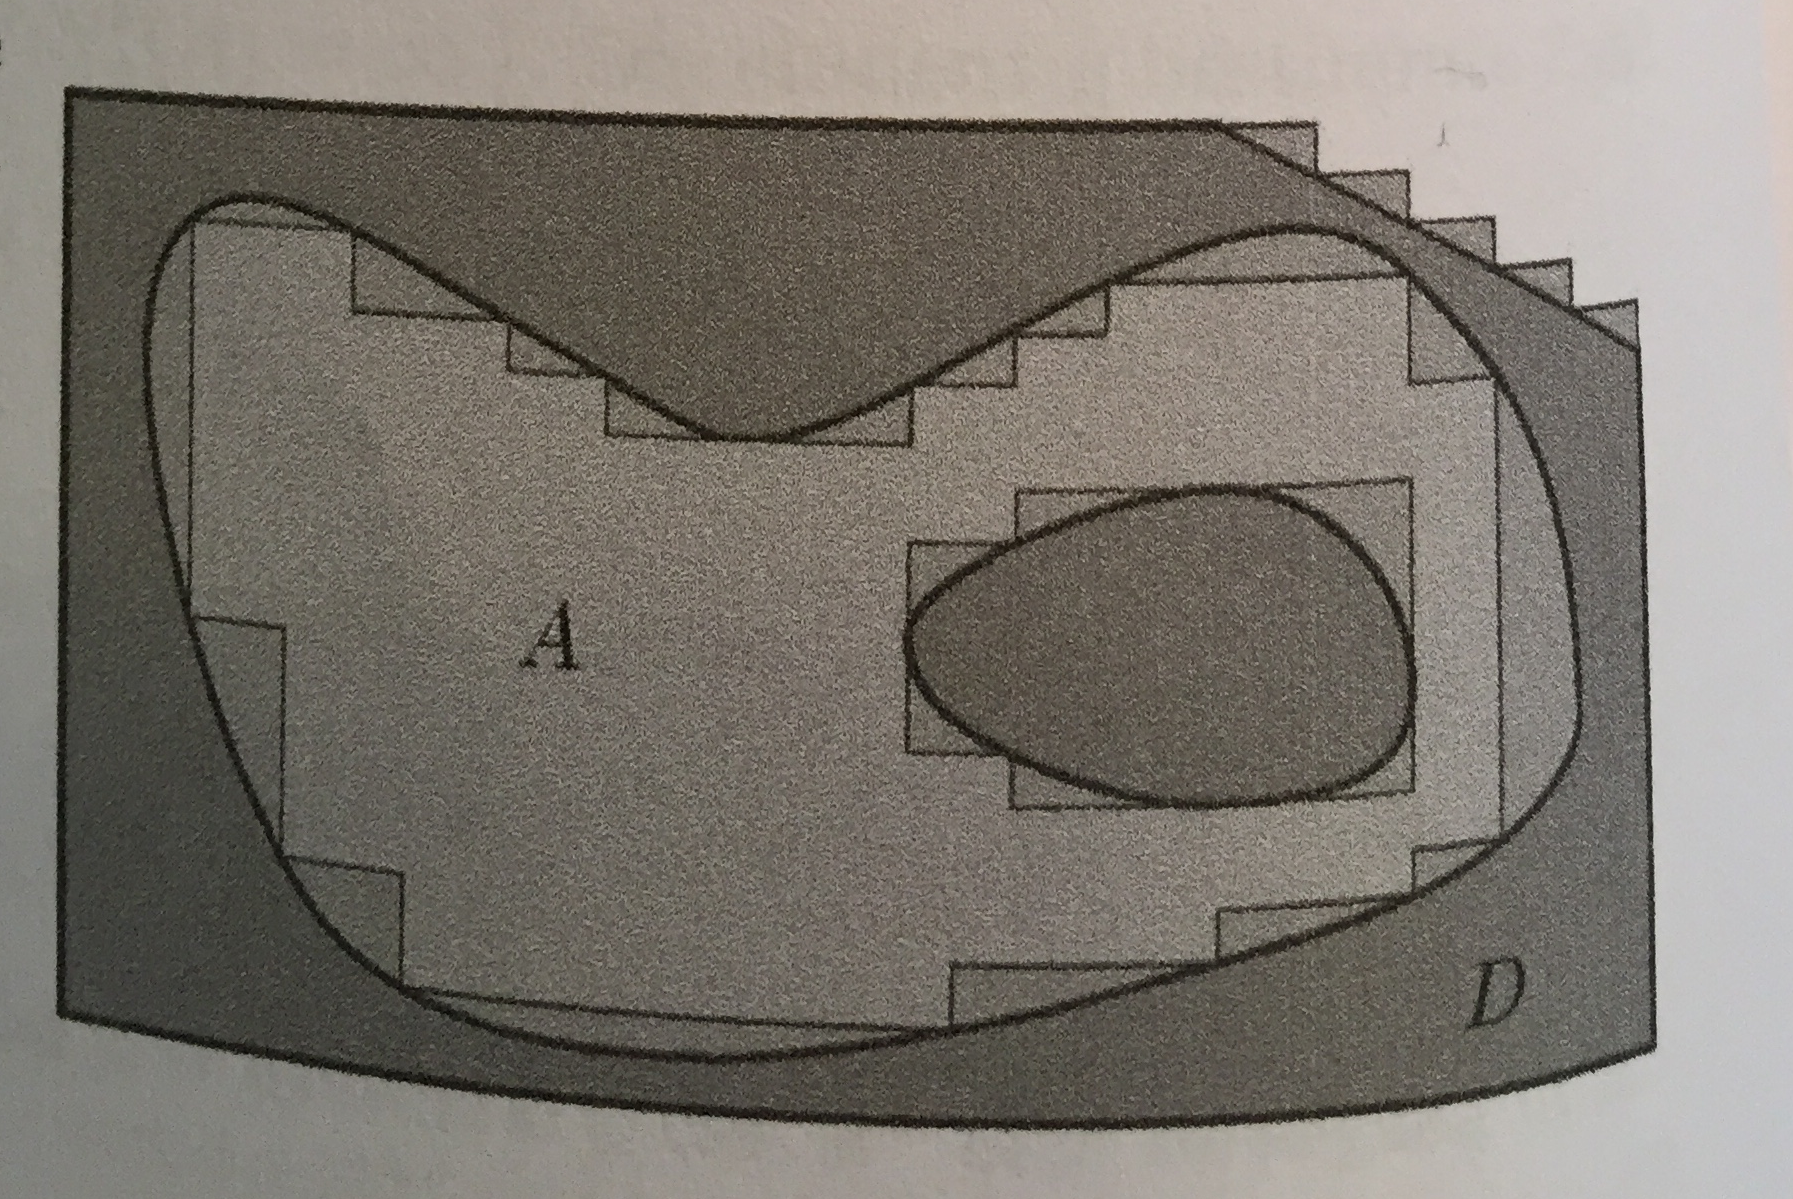
\includegraphics[width=1.0\textwidth]{images/im}
    \caption{Inneres Maß}
  \end{minipage}
\end{figure}

Es ist daher sinnvoll von einer messbaren Menge zu sprechen, wenn diese beiden Volumen übereinstimmen, also
$\mu_D(A) = \mu(A)$ gilt. Dies ist gleichbedeutend mit der Bedingung $\mu(D) = \mu(A) + \mu(D  \setminus A)$. 
Für festes $D$ wären somit alle Mengen $A$ messbar, für die das äußere Lebesgue Maß additiv ist auf der Zerlegung $D = A \cup D \setminus A$. 
Lässt man die Bedingungen der Beschränktheit und $A \subset D$ fallen, gelangt man zu folgender Definition.

\begin{Definition}[$\mu$-messbare Menge]
Eine Menge $A \subset \mathbb{R}^n$ heißt messbar, falls für alle $D \subset  \mathbb{R}^n$ gilt
\begin{align*}
\mu(D) =  \mu(A \cap D) + \mu(A^c \cap D)
\end{align*}
Da wir die $\sigma$-subadditivität bereits nachgewiesen haben, können wir diese Bedingung auf
\begin{align*}
\mu(D) \geq  \mu(A \cap D) + \mu(A^c \cap D)
\end{align*}
reduzieren. Die Menge aller messbaren Mengen bezeichnen wir mit $\mathcal{A}$.
\end{Definition}

\begin{Bemerkung}
Nullmengen sind messbar.
\end{Bemerkung}
\begin{proof}
Es sei $N, D \subset \mathbb{R}^n$ mit $\mu(N)= 0$. Wegen der Monotonie von $\mu$ ist $0 \leq \mu (N \cap D) \leq \mu(N) = 0$ und somit ist $N \cap D$ auch eine Nullmenge. Wir erhalten damit und nochmaliger Monotonie von $\mu$
$$ \mu(N \cap D) + \mu (N^c \cap D) =  \mu (N^c \cap D) \leq \mu(D) $$
und damit ist $N$ messbar.
\end{proof}



\subsubsection*{$\sigma$-Algebra der messbaren Mengen}
Die Menge der messbaren Mengen $\mathcal{A}$ hat einige besondere Eigenschaften. Wir geben hier nur diese Eigenschaften ohne Beweis an. Die Beweise verwenden im wesentlichen Techniken, die wir bereits kennengelernt haben.
\begin{itemize}
\item Für eine Folge $A_i \in \mathcal{A}$ von messbaren Mengen mit $A_i \cap A_j  =  \emptyset$ ist $\mu (\bigcup_i A_i ) = \sum_i \mu(A_i)$.
\item Ist $A \in \mathcal{A} $, so ist auch $A^c \in \mathcal{A} $.
\item Für eine Folge $A_i \in \mathcal{A}$ messbarer Mengen  ist $\bigcup_i A_i \in \mathcal{A}$ messbar.
\end{itemize}



\begin{Satz}[Charakterisierung messbarer Mengen]
Eine Menge $A$ ist genau dann messbar, wenn $A = S \cup N$, wobei $N$ eine Nullmenge und $S$ Vereinigung von kompakten Mengen ist.
\end{Satz}


\subsection{Lebesgue Integral}

\begin{Definition}
Für eine Teilmenge $A \subset \mathbb{R}^n$ heißt
$$ 1_A (x): = \begin{cases} 1 \text{  falls }   x \in A  \\  0  \text{  sonst}  \end{cases}$$
Indikatorfunktion.
\end{Definition}

\begin{Definition}
Eine Funktion 
$$ \varphi(x) := \sum_{k=1}^m c_k 1_{I_k}$$ mit $c_k \in \mathbb{R}$ und $I_k \in \mathbb{I}(n)$ mit $I_l \cap I_h = \emptyset$ für $i \neq j$
heißt Treppenfunktion.
\end{Definition}

\begin{figure}[H]
      \centering
    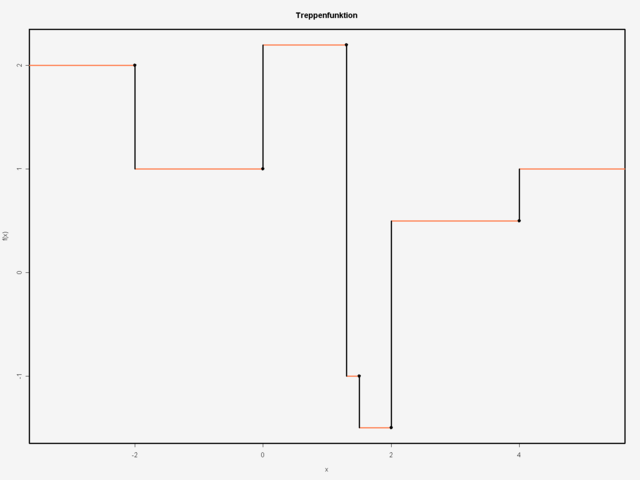
\includegraphics[width=0.8\textwidth]{images/640px-Stepfunction1}
      \caption{Quelle: Wikipedia: https://commons.wikimedia.org/wiki/File:Stepfunction1.png}

\end{figure}



\begin{Bemerkung}
Seien $\varphi(x) =   \sum_{k=1}^m  c_k 1_{I_k}$ und $\psi(x) =  \sum_{j=1}^l  u_j 1_{I_j}$. Dann definiert
$(\varphi + \psi)(x) := \sum_{k=1}^m \sum_{j=1}^l   (c_k + u_j) 1_{I_{k,j}}$ mit $I_{k,j}:= I_k \cap I_j$ eine Treppenfunktion (nach entsprechender Umnummerierung zu einem einzigen Summenzeichen).
\end{Bemerkung}


\begin{Definition}
Für eine Treppenfunktion $ \varphi(x) := \sum_{k=1}^m c_k 1_{I_k}$ definieren wir das Integral durch
$$\int_{\mathbb{R}^n} \varphi d\mu := \sum_{k =1}^m  c_k \mu(I_k) \; . $$
\end{Definition}

\begin{Satz}
\label{TFB}
Seien $\varphi(x) =   \sum_{k=1}^m  c_k 1_{I_k}$ und $\psi(x) =  \sum_{j=1}^l  u_j 1_{I_j}$ zwei Treppenfunktionen.
Für das Integral von Treppenfunktion gilt:
\begin{itemize}
\item Ist $\varphi(x) = \psi(x)$ für alle $x$, dann ist $\int_{\mathbb{R}^n} \varphi d\mu = \int_{\mathbb{R}^n} \psi d\mu$ (Das integral hängt nicht von der Zerlegung der Treppenfunktion ab und  ist wohldefiniert)
\item $\int_{\mathbb{R}^n} \alpha \varphi  + \beta \psi d\mu = \alpha \int_{\mathbb{R}^n}  \varphi d\mu + \beta  \int_{\mathbb{R}^n}  \psi d\mu$
\item $ \biggl|  \int_{\mathbb{R}^n} \varphi d\mu  \biggr| \leq \int_{\mathbb{R}^n} | \varphi | d\mu$
\item Ist $\varphi(x) \leq \psi(x)$ für alle $x$, so ist $\int_{\mathbb{R}^n} \varphi d\mu \leq \int_{\mathbb{R}^n} \psi d\mu$ 
\end{itemize}
\end{Satz}

\begin{proof}
Der Beweis wird über eine vollständige Induktion geführt. Der Induktionsanfang ist einfach zu zeigen. 
Wir nehmen an, die Aussage gilt für alle Dimensionen $k < n$.
Zerlege $\mathbb{R}^n = \mathbb{R}^p \times \mathbb{R}^{n-p}$. Jeder Quader $I \in \mathbb{I}(n)$ zerlegt sich damit ebenfalls in ein Produkt 
$I = I' \times I''$ mit $I'  \in \mathbb{I}(p)$ und  $I''  \in \mathbb{I}(n-p)$ und für $z = (x,y) \in  \mathbb{R}^p \times \mathbb{R}^{n-p}$ gilt $1_{I} (z) = 1_{I'}(x) \cdot 1_{I''}(y)$. Es sei nun $\varphi(z):=   \sum_{k=1}^m  c_k 1_{I_k}(z)$ eine Treppenfunktion auf $ \mathbb{R}^p \times \mathbb{R}^{n-p}$. Für jedes $y \in \mathbb{R}^{n-p}$ definiert  $\varphi_y(x)=   \sum_{k=1}^m  c_k 1_{I''_k}(y) \cdot 1_{I'_k}(x)$ eine Treppenfunktion auf $\mathbb{R}^{n-p}$. 
Nach Induktionsvoraussetzung hängt das Integral 
$$\int_{\mathbb{R}^p}  \varphi_y(x) d \mu' = \sum_{k=1}^m  c_k \mu'(I'_k)  \cdot 1_{I''_k}(y)  =: \phi(y)$$
nicht von der Zerlegung der Treppenfunktion ab. $\phi(y)$ ist wiederum eine Treppenfunktion auf $\mathbb{R}^{n-p}$ und Nach Induktionsvoraussetzung hängt das Integral 
$$\int_{\mathbb{R}^{n-p}}  \phi(y) d \mu'' = \sum_{k=1}^m  c_k \mu'(I'_k)  \cdot \mu'' (I''_k)(y) $$
nicht von der Zerlegung der Treppenfunktion ab. Somit gilt
$$\int_{\mathbb{R}^{n-p}} \int_{\mathbb{R}^p}  \varphi_y(x) d \mu'  d \mu''  =   \sum_{k=1}^m  c_k \mu'(I'_k)  \cdot \mu''(I''_k)(y) = \sum_{k=1}^m  c_k  \mu(I_k)  = \int_{\mathbb{R}^n} \varphi(z) d\mu\;.$$
Die linke Seite hängt  damit nicht von der Zerlegung der Treppenfunktion ab und alle Behauptungen können so auf den Fall $n=1$ zurückgeführt werden.
\end{proof}

\begin{Bemerkung}[Satz von Fubini für Treppenfunktionen]
\label{FTF}
Es gilt $$\int_{\mathbb{R}^n} \varphi(x,y) d \mu = \int_{\mathbb{R}^{n-p}} \biggl (\int_{\mathbb{R}^{p}}  \varphi(x,y) d \mu' \biggr ) d \mu''$$
\end{Bemerkung}
\begin{proof}
Siehe Beweis des letzten Satzes.
\end{proof}


\subsubsection{Die $L^1$-Halbnorm}
Der Fall $\infty$ ist bei den folgenden Betrachtungen immer als möglicher Fall zu berücksichtigen.

\begin{Definition}
Eine Hüllreihe zu einer Funktion $f :\mathbb{R}^n \to \mathbb{R}$ ist eine Reihe $\phi(x):= \sum_{k=1}^{\infty} c_k  1_{I_k} (x)$ mit den folgenden Eigenschaften:
\begin{itemize}
\item $c_k \in \mathbb{R}$ sind positive reelle Zahlen $c_k >0$.
\item $I_k \subset \mathbb{R}^n$ sind offene Quader.
\item Für alle $x \in \mathbb{R}^n$ gilt $|f(x) | \leq \phi(x)$.
\end{itemize}
\end{Definition}


\begin{Definition}
Der Innhalt einer Hüllreihe $\phi(x):= \sum_{k=1}^{\infty} c_k  1_{I_k} (x)$ ist definiert durch 
$$I (\phi) := \sum_{k=1}^{\infty} c_k \;  \mu(I_k) \; .$$
\end{Definition}


\begin{Definition}
Die $L^1$-Halbnorm einer Funktion $f :\mathbb{R}^n \to \mathbb{R}$ is definiert durch das Infimum der Inhalte der Hüllreihen zu $f$
$$ || f ||_1 : = \inf  \biggl \{   I(\phi) \; | \; \phi  \text{ ist Hüllreihe zu  }  f \biggr \} \; .$$
\end{Definition}

\begin{Lemma}[Verallgemeinerte Dreiecksungleichung]
\label{vdug} 
Für nicht negative Funktionen $f_k  :\mathbb{R}^n \to \mathbb{R}_{\geq 0}$ gilt
$$ \biggl | \biggl | \sum_{k=1}^{\infty} f_k \biggr | \biggr |_1 \leq  \sum_{k=1}^{\infty} || f_k  ||_1 \; .$$
\end{Lemma}

\begin{proof}
Zu $\epsilon > 0$ und $f_k$ wählen wir eine Hüllreihe $\phi_k = \sum_{i} c_{ik} 1_{I_{ik}}$ mit Inhalt
$$ I(\phi_k) =  \sum_{i} c_{ik} \; \mu (1_{I_{ik}}) = || f_k||_1 + \frac{\epsilon}{2^k} \;.$$ Dann ist $\phi := \sum_{k,i} c_{ik} 1_{I_{ik}}$ eine Hüllreihe der Funktion $\sum_k f_k$ mit 
$$ I(\phi) = \sum_{k,i} c_{ik}  \; \mu (I_{ik}) = \sum_k \biggl( \sum_i  c_{ik} \; \mu (I_{ik})\biggr) \leq \sum_k || f_k ||_1 + \epsilon$$
Mit  $ \bigl | \bigl | \sum_{k=1}^{\infty} f_k \bigr | \bigr |_1 \leq I(\phi) $ und $\epsilon \to 0$ folgt die Behauptung.
\end{proof}

\begin{Bemerkung}[Rechenregeln]
Für $f,g : \mathbb{R}^n \to \mathbb{R}$ und $c \in \mathbb{R}$ gilt:
 \begin{itemize}
\item $|| cf ||_1 \leq |c| || f ||_1$. 
\item $|| f +g ||_1 \leq  ||f ||_1 + ||g||_1$
\item Aus $|| f (x)||_1 \leq g(x)$ für alle $x$ folgt $|| f ||_1 \leq || g ||_1$.
\end{itemize}
\end{Bemerkung}
\begin{proof}

 \begin{itemize}
\item Für eine Hüllreihe $\varphi$ von $f$ ist $|c| \cdot \varphi$ eine Hüllreihe von $c \cdot f$. 
\item  Da $|f +g | \leq | f | + | g |$ folgt Behauptung aus (iii) und der verallgemeinerten Dreiecksungleichung.
\item Hullreihen sind immer größer-gleich der Funktion und damit haben größere Funktionen größere Hüllreihen.
\end{itemize}
\end{proof}

\begin{Lemma}[Fundamentallemma]
Für die charakteristische Funktion $1_{I}$ eines Quaders $I$ gilt 
$$ || 1_I ||_1 = \mu(I) =  \text{vol} (I) = \int 1_I d \mu$$
\end{Lemma}
\begin{proof}
$ 1 \cdot 1_I$ ist eine Hüllfunktion von $1_i$ und damit gilt $|| 1_I || \leq \mu(I)$. 
Sei $\phi(x) = \sum_k c_k 1_{I_k} $ eine Hüllreihe von $1_i$ und $\epsilon >0$. Da $\phi(x) \geq 1$ gibt es für jedes $x$ einen Index $N(x)$ mit 
$\sum_{k=1}^{N(x)} c_k 1_{I_k} \geq 1 - \epsilon$. Da die $I_k$ offen sind, gibt es für jedes $x$ eine Umgebung $U(x)$, so dass letztere Gleichung gilt. Da $\bar{I}$ kompakt ist (beschränkt und abgeschlossen), überdecken endlich viele $U(x_1), \cdots , U(x_n)$ den Quader $I$. Mit $N:= \max \{ N(x_1), \cdots , N(x_n)$ folgt $\sum_{k=1}^N c_k 1_{I_k} \geq (1-\epsilon) 1_I$. Aus Satz \ref{TFB} (iii) folgt
$$ I (\phi) = \sum_k c_k \mu(I_k) \geq \sum_{k=1}^N c_k \mu (I_k) \geq (1 - \epsilon) \mu(I) \;.$$
Mit $\epsilon \to 0$ folgt $I (\phi) \geq \mu(i)$ und damit insgesamt die Behauptung.  
\end{proof}


\begin{Lemma}
\label{normbetragintegral}
Für jede Treppenfunktion $\varphi$ auf $\mathbb{R}^n$ gilt
$$ || \varphi ||_1 = \int | \varphi | d \mu  \; .$$
\end{Lemma}


\subsubsection{Integration über den $\mathbb{R}^n$}

\begin{Definition}
Eine Funktion $f : \mathbb{R}^n \to \mathbb{R}$ heißt integrierbar, falls eine Folge von Treppenfunktionen  $\varphi_k$ existiert mit
$$ || f -  \varphi_k ||_1 \to 0 \text{ für } k \to \infty \;. $$
In diesem Fall heißt
$$ \int_{\mathbb{R}^n} f(x) d \mu := \lim_{k \to \infty} \varphi_k d \mu$$
das Integral von $f$ über $\mathbb{R}^n$.
\end{Definition}

\begin{Bemerkung}
\hfill
\begin{itemize}
\item Die reelle Zahlenfolge $\int \varphi_k d\mu$ ist eine Cauchyfolge und damit konvergent. 
\item Der Grenzwert ist unabhängig von der Folge $\varphi_k$.
\end{itemize}

\end{Bemerkung}
\begin{proof}
Für Treppenfunktionen $\psi$ und $\xi$ gilt 
\begin{align*}
\biggl | \int \psi d \mu - \int \xi d \mu \biggr |  &  \leq \int | \psi - \xi | d \mu = || \psi - \xi ||_1 \\
& \leq  || \psi - f ||_1 +  || f - \xi ||_1
\end{align*}
woraus die Behauptungen folgen.
\end{proof}

\begin{Satz}
\label{ibf}
Ist $f$ über $\mathbb{R}^n$ integrierbar, so auch $|f|$ und es gilt
$$ \biggl | \int f d \mu \biggr | \leq \int  | f | d \mu = || f ||_1 \; .$$
\end{Satz}
\begin{proof}
Sei $f$ integrierbar und $\varphi_k$ eine Folge von Treppenfunktionen mit $|| f - \varphi_k ||_1 \to 0$. 
Aus $\bigl | | f | - | \varphi_k | \bigr | \leq | f -\varphi | $ ergibt sich wegen der Monotonie der $L^1$-Norm
$$\bigl |  \bigl |  | f | - | \varphi_k | \bigr | \bigr |_1 \leq \bigl |  \bigl |   f  -  \varphi_k  \bigr | \bigr |_1  \; .$$ 
Damit gilt $\bigl |  \bigl |  | f | - | \varphi_k | \bigr | \bigr |_1 \to 0$ und somit ist $|f|$ integrierbar und mit der Abschätzung von Beträgen für Treppenfunktionen aus Satz \ref{TFB} gilt 
\begin{align*}
\biggl | \int f d \mu \biggr | = \biggl | \lim_k \int \varphi_k d \mu \biggr | \leq  \int |\varphi_k| d \mu = \int |f| d\mu
\end{align*} 
und damit der erste Teil der Behauptung. 
Mit der Dreiecksungleichung erhalten wir
$$ || f || - ||  f - \varphi ||_1 \leq || \varphi_k ||_1  \leq || f ||_1 + || f - \varphi_k ||_1 $$
und wegen $|| \varphi_k ||_1 = \int | \varphi_k | d \mu \to \int | f | d \mu$ folgt die Behauptung.
\end{proof}


\begin{Bemerkung}[Rechenregeln]
Sind $f$ und $g$ integrierbar, so gilt
\begin{itemize}
\item $ \alpha f + \beta g$ mit $\alpha, \beta \in \mathbb{R}$ ist integrierbar mit 
$$\int \alpha f + \beta g d\mu = \alpha \int f d\mu + \beta \int g d \mu \; .$$ 
\item Aus $f(x) \leq g(x)$ für alle $x \in \mathbb{R}^n$ folgt $\int f d \mu \leq \int g d \mu$.
\item Ist $g$ zusätzlich beschränkt, so ist auch $f \cdot g$ integrierbar.
\end{itemize}
\end{Bemerkung}
\begin{proof}
\begin{itemize}
\item Sind $\phi_k$ und $\psi_k$ approximierende Folge von  Treppenfunktionen von $f$ und $g$, so ist $\alpha \phi_k + \beta \psi_k$ eine approximierende Folge von $\alpha f + \beta g$.
\item Nach Satz \ref{ibf} ist $\int (g-f) d \mu = || g - f ||_1 \geq 0$.
\end{itemize}
\end{proof}


\begin{Bemerkung}
Ist $f$ integrierbar, so auch $f^+ := \max(f,0)$ und $f^- := \min(f,0)$. Damit ist $f = f^+ + f^-$ genau dann integrierbar, wenn $f^+$ und $f^-$ integrierbar sind. Da $- f^- \geq 0$ ist, kann man sich in Beweisen häufig auf den Fall $f \geq 0$ beschränken.
\end{Bemerkung}
\begin{proof}
Es ist $ \max(f,0) = \frac{1}{2} (f + | f |)$ und  $ \min(f,0) = \frac{1}{2} (f - | f |)$ und die Behauptung folgt aus den Rechenregeln.
\end{proof}

\begin{Definition}[Integration über Teilmengen]
Für  eine Teilmenge $A \subset \mathbb{R}^n$ und eine Funktion $f: A \to \mathbb{R}$ heißt
$$  f_A (x) : = \begin{cases}  f(x) \text{ für } x \in A \\ 0  \text{ für } x \in \mathbb{R}^n \setminus A \end{cases}$$ 
die triviale Fortsetzung von $f$ auf $\mathbb{R}^n$. $f$ heißt integrierbar über $A$, falls $f_A$ über $\mathbb{R}^n$ integrierbar ist und in diesem Fall bezeichnen wir mit $$ \int_A f(x) d \mu := \int f_A (x) d\mu$$ als das Integral von $f$ über $A$.
\end{Definition}




\begin{Satz}[Kleiner Satz von B. Levi]
\label{KBL}
Zu $f: \mathbb{R}^n \to \mathbb{R}$ gebe es eine monoton wachsende Folge $\varphi_k$ von Treppenfunktionen mit
\begin{itemize}
\item Für alles $x \in \mathbb{R}^n$ git $\lim_{k \to \infty} \varphi(x) =  f(x)$. $f$ ist also die punktweise gebildete Grenzfunktion der $\varphi_k$.
\item Die reelle Folge der Integrale $\int \varphi_k d \mu $ ist beschränkt.
\end{itemize}
Dann ist $f$ integrierbar und es gilt

$$ \int f d \mu = lim_{k \to \infty}  \int \varphi_k d \mu \; .$$
\end{Satz}

\begin{proof}
Aus $f - \varphi_k = \sum_{i=k}^{\infty} (\varphi_{k+1} - \varphi_k)$ folgt mit der verallgemeinerten Dreiecksungleichung Lemma \ref{vdug}  und Lemma \ref{normbetragintegral}
\begin{align*}
|| f - \varphi_k ||_1 \leq \sum_{i=k}^{\infty} \int | \varphi_{i+1} - \varphi_i | d \mu =  \sum_{i=k}^{\infty} \biggl ( \int  \varphi_{i+1}d \mu -  \int \varphi_i  d \mu \biggr ) \; .
\end{align*}
Die Folge $\int \varphi_k$ ist monoton wachsend und beschränkt und damit konvergent. Bezeichnen wir mit $I$ den Grenzwert, so folgt 
$|| f -\varphi_k ||_1 \leq I - \int \varphi_k d \mu $. Also gilt $|| f -\varphi_k ||_1 \to 0$ für $k \to \infty$ und damit ist $f$ integrierbar und mit der Definition des Integrals folgt die Behauptung.
\end{proof}


\begin{Definition}
Eine Menge $U \subset \mathbb{R}^n$ heißt offen, falls für alle $a \in U$ ein Radius $r >0$ existiert, so dass der Ball $B_r(a) : = \{ x \in \mathbb{R}^n \; | \; ||x -a|| \leq r \} \subset U$ in $U$ enthalten ist.
\end{Definition}

\begin{Satz}
\label{fintu}
Sei $U \subset \mathbb{R}^n$ offen und beschränkt und $f : U \to \mathbb{R}$ stetig und beschränkt. Dann ist $f$ über $U$ integrierbar.
\end{Satz}

\begin{proof}
Da $U$ offen ist, kann  man um jeden Punkt $a \in U$ einen Würfel $W_r(a)$ finden, dessen Mittelpunkt $a$  und dessen Kantenlänge $r$ eine rationale Zahl ist. Damit kann man zu Punkten $a_1, \cdots,  a_n$ Würfel wählen, so dass $W_r(a_i) \cap W_r(a_j) = \emptyset$ für $i \neq j$ und mit $m_i := \min \{ f(x)  | x \in W_r(a_i) \} $ Hüllreihen   $\psi_{a_1, \cdots, a_n} := \sum_{i=1}^n m_i 1_{W_r(a_i)} $  konstruieren mit  $\psi \leq f$. Bezeichnen  wir mit $\mathcal{T} :=  \{ \psi_k  \}$ die abzählbare Menge dieser Treppenfunktionen, so ist $f = \sup \{ \psi \; | \; \psi \in \mathcal{T}  \}$ und $\varphi_k : = max \{ \psi_1, \cdots \psi_k  \}$ eine monoton wachsende Treppenfunktion mit $\varphi_k \to f$. Da $U$ beschränkt ist, gibt es eine Quader $I$ mit $U \subset I$ und mit $M : = \max (f)$  ist $\int \varphi_k d \mu \leq M \mu(I)$ beschränkt. Mit dem Satz von B. Levi folgt die Behauptung. 
\end{proof}


\begin{Satz}[Schnittmenge]
Sei $ A \subset \mathbb{R}^n$. Für $ y \in \mathbb{R}^p$ heißt
$$ A_y :=  \biggl \{    x \in \mathbb{R}^{n-p}  \; | \;  (x,y) \in A \biggr \}$$  
Schnittmenge von $A$ zu $y$.
\end{Satz}


\begin{Satz}[Kleiner Satz von Fubuni]
Sei $A \subset \mathbb{R}^n$ eine offene und beschränkte Teilmenge und $f : U \to \mathbb{R}$  eine stetige und beschränkte Funktion.
Dann ist für jedes $ y \in \mathbb{R}^p$ mit $A_y \neq \emptyset$ die Funktion $f_y(x) := f(x,y)$ über $A_y$ und   
$$ F(y) := \begin{cases}   \int_{A_y} f(x,y) d \mu_{p}  , \text{ falls }  A_y \neq \emptyset 
\\ 0 \text{ sonst } \end{cases} $$
über $\mathbb{R}^{p}$ integrierbar und es gilt 
$$ \int_A f(x,y) d \mu_n = \int_{\mathbb{R}^p}  \int_{\mathbb{R}^p } F(y) d \mu_p \; .$$
 Hierfür schreiben wir auch kurz
$$ \int_A f(x,y) d \mu_n  = \int_{\mathbb{R}^{p} }  \biggl ( \int_{A_y} f(x,y)  d\mu_{n-p} \biggr ) d\mu_p$$
\end{Satz}
\begin{proof}
Wie in Beweis zu Satz \label{fintu} sei  $\varphi_k$ eine monoton wachsende Folge von Treppenfunktionen auf $\mathbb{R}^n$ mit $|| f_A - \varphi_k ||_1 \to 0$.
Für jedes $y \in \mathbb{R}^p$ bilden dann die Funktionen $\varphi_k(x)_y := \varphi_k(x,y)$ eine monoton wachsende Folge von Treppenfunktionen auf $\mathbb{R}^{n-p}$, die gegen $f_y(x):= f_A(x,y)$ konvergiert. Die Folge der Integrale $\int_{\mathbb{R}^{n-p}} \varphi_k(x)_y d \mu_{n-p}$ ist beschränkt,  da $A$ beschränkt ist, und daher gibt es eine Quader $I$ mit $U \subset I$ und  mit $M : = \max (f)$  ist $\int \varphi_k d \mu \leq M \mu(I)$ beschränkt. Mit dem kleinen Satz von B. Levi \ref{KBL}
gilt
$$ F(y) := \lim_{k \to \infty} \int_{\mathbb{R}^{n-p}} \varphi_k(x)_y d \mu_{n-p} \; .$$
Die Funktionen 
$$\phi_k (y) := \int_{\mathbb{R}^{n-p}} \varphi_k (x,y) d \mu_{n-p}$$
sind Treppenfunktionen auf $\mathbb{R}^{p}$ und die Folge $\phi_k$ konvergiert monoton wachsend gegen $F$ und die Folge der Integrale 
$\int \phi_k(y) d \mu_{p}$ ist beschränkt, da  mit dem Satz von Fubini für Treppenfunktionen \ref{FTF} und $\varphi_k \leq f_A$  
$$ \int_{\mathbb{R}^{p}} \phi_k(y) d \mu_{p} = \int_{\mathbb{R}^n} \varphi_k(x,y) d\mu_{n} \leq \int_{\mathbb{R}^n} f_A(x,y) d \mu_{n} \; .$$
Mit dem kleinen Satz von B. Levi ist $F$ integrierbar und es gilt
\begin{align*}
 \int_{\mathbb{R}^{p}}   F(y) d \mu_{p} & = \lim_{k \to \infty}  \int_{\mathbb{R}^{p}}  \phi_k (y) d \mu_{p} =  \lim_{k \to \infty}  \int_{\mathbb{R}^{n}}  \varphi_k(x,y) d \mu_{n} \\
& =   \int_{\mathbb{R}^{n}}  f_A (x,y) d \mu_{n}  \; .
\end{align*} 
\end{proof}


\begin{Satz}[Lebesgue vs. Riemann]
Eine \href{https://de.wikipedia.org/wiki/Regelfunktion}{Regelfunktion} $f$ auf $[a,b] \subset \mathbb{R}$ ist über $[a,b] $ Lebesgueintegrierbar und es gilt 
\begin{align*}
\int_{[a,b]} f(x) d \mu_1 = \int_a^b f(x) dx \; .
\end{align*}
\end{Satz}
\begin{proof}
Sei $\varphi_k$ eine Folge von Treppenfunktionen mit $|| f -\varphi_k ||_{\infty} \to 0$. Da für jede Funktion $h$ auf $[a,b]$ die Abschätzung
$|h| \leq || h ||_{\infty} 1_{[a,b]}$ gilt, folgt auch $$|| f_A -\varphi_{k,A} ||_{1} \to 0$$ und damit ist $f_{[a,b]}$ auch Lebesgueintegrierbar über $[a,b]$ mit Lebesgueintegral
\begin{align*}
\int_{[a,b]} f(x) d \mu= \int_{\mathbb{R}} f_A(x) d\mu = \lim_k \varphi_{k,A} d \mu = \lim_k \int_a^b \varphi_k dx = \int_a^b f (x) dx
\end{align*}
 
\end{proof}

\begin{Beispiel} [Integration über Kreis]
Sei $K := B^2_1(0) := \{   (x,y) \in \mathbb{R}^2 \; | \; \sqrt{x^2 + y^2 } \leq 1\}$. Mit dem kleinen Satz von Fubini erhalten wir
\begin{align*}
\int_K 1 d \mu = &  \int_{-1}^{1} \biggl ( \int_{-\sqrt{1- y^2}}^{\sqrt{1- y^2}} 1 dx \biggr ) dy = \\ 
& =  2 \int_{-1}^{1}  \sqrt{1 - y^2}   \; dy  \\ 
 & (substitution \;   y = sin(u)) =   2 \int_{-\frac{\pi}{2}}^{\frac{\pi}{2}}   \cos(u)^2   \; du = 2 \cdot \frac{\pi}{2} = \pi
\end{align*}
\end{Beispiel}
\begin{figure}[H]
      \centering
    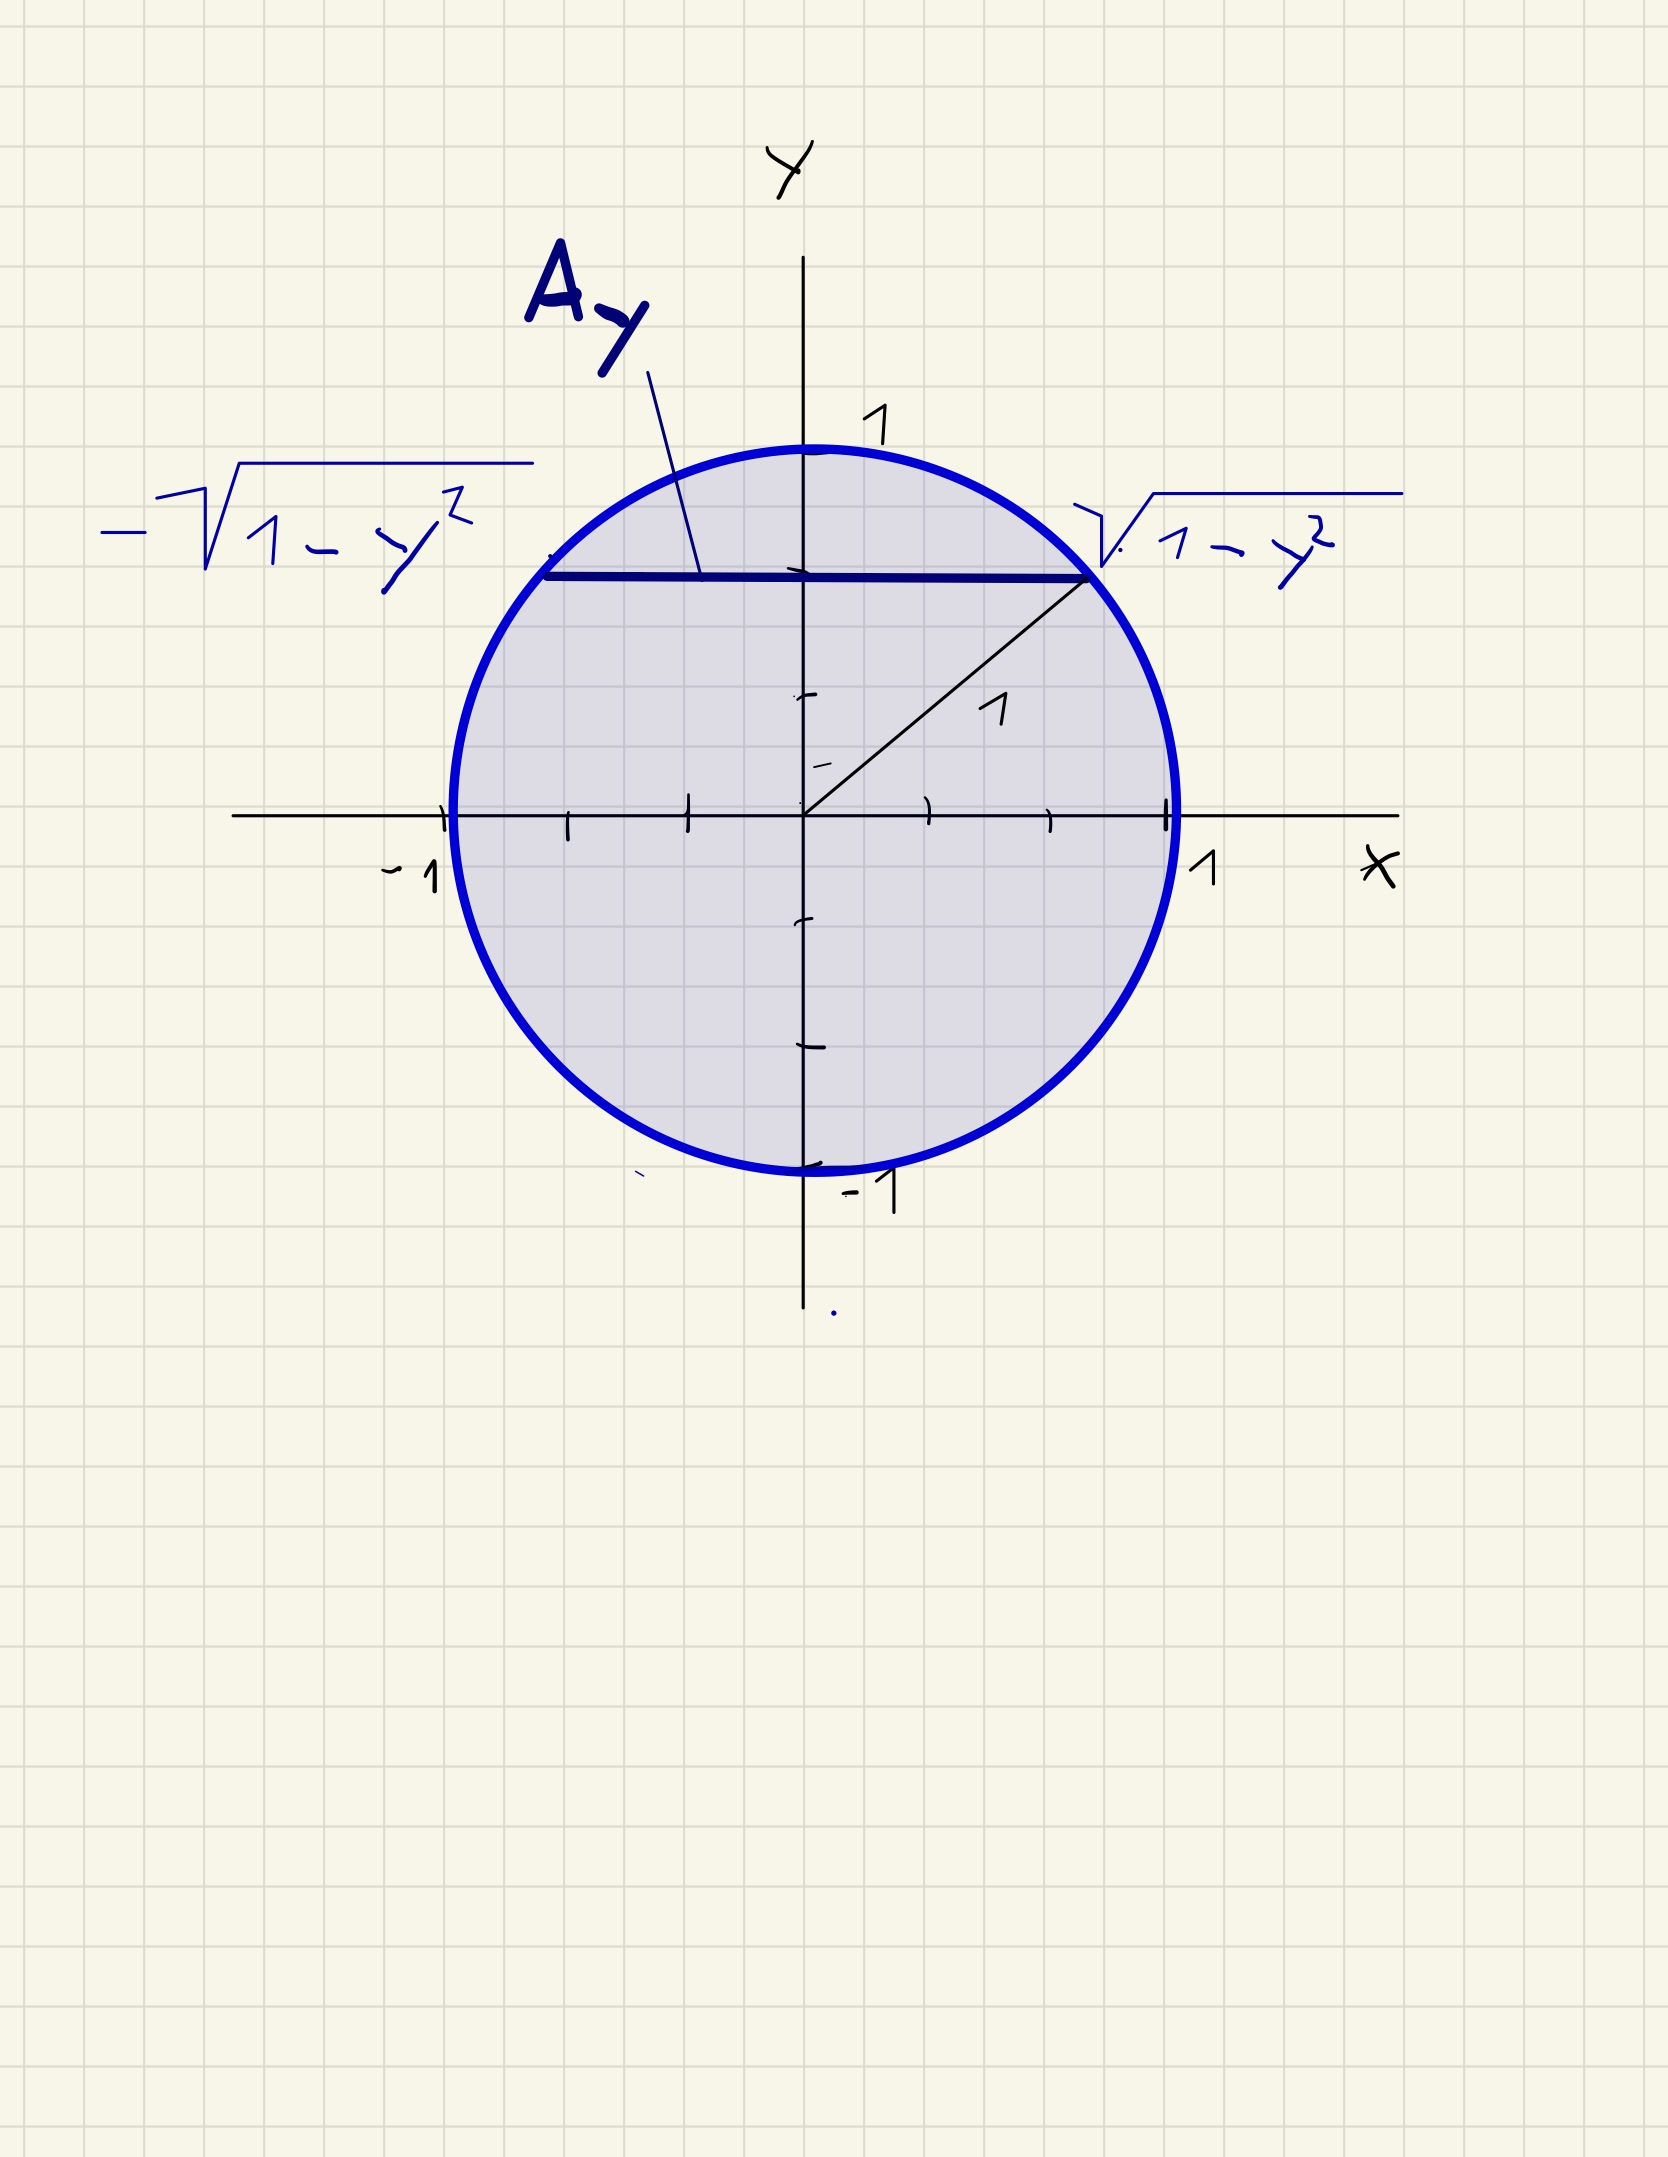
\includegraphics[width=0.8\textwidth]{images/Kreis}
\end{figure}


\subsubsection{Transformationssatz}




\begin{Satz}
Seien $U$ und $V$ offene Teilmengen des $\mathbb{R}^n$, $T': U \to V$ ein lineare Abbildung und  $Q \in \mathbb{I}(n)$ ein Quader.
Dann gilt:
 $$ \text{vol}  (T'(Q))   =  \det (T') \cdot   \text{vol}(Q) \; .$$
\end{Satz}
\begin{proof}
Für Vektoren $a_1, \cdots a_n$ im $\mathbb{R}^n$ heißt die Menge 
$$ P(a_1, \cdots,  a_n) := \biggl \{  x = \sum_{k=1}^n t_k a_k  \; | \; t_1, \cdots , t_n \in [0,1]  \biggr \}$$
Parallelotop.
\begin{figure}[H]
      \centering
    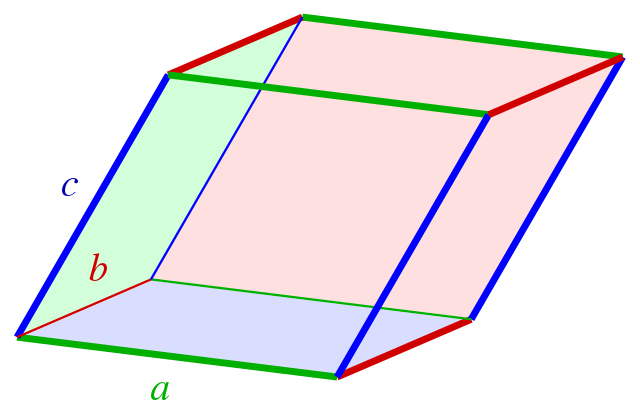
\includegraphics[width=0.6 \textwidth]{images/640px-Parallelepiped-0}    
\end{figure}
Es gilt  $$  \text{vol} \bigr( P(a_1, \cdots, a_n) \bigr) =  | det (a_1, \cdots, a_n) |   \; .$$

\href{https://www.math.uchicago.edu/~may/VIGRE/VIGRE2007/REUPapers/FINALAPP/Peng.pdf}{Ausfürlicher Beweis}

\end{proof}


\begin{Definition}[Diffeomorphismus]
Seien $U$ und $V$ offene Teilmengen des $\mathbb{R}^n$. Eine Abbildung  $T: U \to V$ heißt diffeomorphismus, wenn eine  Umkehrfunktion $T^{-1}: V  \to U$ existiert, also $T^{-1} (T (u)) = u$ gilt für alle $u \in U$, die ebenfalls differenzierbar ist.
\end{Definition}

\begin{Beispiel}
Für eine invertiertere Matrix $A$ ist $T(x):= Ax$ ein Diffeomorphismus.
\end{Beispiel}

\begin{Satz}
Seien $U$ und $V$ offene Teilmengen des $\mathbb{R}^n$, $T: U \to V$ ein Diffeomorpismus und $f: V \to \mathbb{R}$ eine integrierbare Funktion. Dann gilt:
$$ \int_V  f(y)  d \mu = \int_U f(T (x))  \cdot | \det(T' (x)) | d \mu   \; .$$
\end{Satz}
\begin{proof}
Seien $I_k \in \mathbb{I}(n)$ Quader, $J_k := T(I_k)$ und $b_k = T(c_k)$. Dann ist 
$$\sum_{k=1}^n  b_k  \text{vol}(J_k) \approx  \sum_{k=1}^n T(c_k) \cdot | \det T' (c_k)|  \text{vol}(I_k) \; .$$
Die Behauptung folgt dann (nicht trivial) durch den Übergang zu Grenzwerten mit entsprechenden Konvergenzsätzen.
\end{proof}

\subsubsection{Parameterabhängige Integrale}

\begin{Definition}
Eine Folge von Funktionen $f_k$ konvergiert Punktweise fast überall gegen eine Funktion $f$, falls es eine Nullmenge $N$ gibt, mit 
$\lim_{k \to \infty} f_k (x) = f(x)$ für alle $x \in \mathbb{R}^n \setminus N$.
\end{Definition}

\begin{Satz}[Satz von Lebesgue]
Sei $f_k$ eine Folge integrierbarer Funktionen auf $\mathbb{R}^n$ die fast überall Punktweise gegen eine Funktion $f$ konvergiert.
Es gebe eine integrierbare Funktion $F$ mit $|f_k (x)| \leq F(x) $ für alle $x \in \mathbb{R}^n$ und alles $k$. Dann ist $f$ integrierbar und es gilt
$$ \int f(x) d \mu = \lim_{k \to \infty} f_k(x) d \mu $$
\end{Satz}

Sei $f: X \times T \subset \mathbb{R}^{n-p} \times \mathbb{R}^p$ eine Funktion, so dass für festes $x \in X$ die Funktion $f_x(t) := f(x,t)$ über $T$ integrierbar ist. Durch Integration erhält man die Funktion 
$$ F(x) := \int_T f(x,t)  d \mu_T$$ 
auf $X$.

\begin{Satz}[Stetigkeitssatz]
$f$ habe zusätzlich die Eigenschaften:
\begin{itemize}
\item Für festes $t$ ist $f_t(x):= f(x,z)$ stetig.
\item Es gibt auf $T$ eine integrierbare Funktion $\phi$ mit $\phi(t) \geq 0$ und $|f(x,t)| \leq \phi(t)$ für alle $(x,t) \in X \times T$.
\end{itemize}
Dann ist die oben definierte Funktion $F$ stetig. 
\end{Satz}
\begin{proof}
Sei  $x_k \to x$   eine konvergente Folge in $X$ und $f_k(t):= f(x_k,t)$. Nach Voraussetzung konvergiert diese Folge Punktweise gegen die Funktion $f_t(x)$ und $| f_k (x) | \leq \phi(x)$. Mit dem Satz von Lebesgue folgt
$$ \lim_{k \to \infty} \int_T f_k(t) d \mu_T = \int_T f(x,t) d \mu_T$$
und damit $ \lim_{k \to \infty} F(x_k) =  F(x)$.
\end{proof}

\begin{Satz}[Differentiationssatz]
$f$ habe zusätzlich die Eigenschaften:
\begin{itemize}
\item Für festes $t$ ist $f_t(x):= f(x,z)$ stetig differenzierbar.
\item Es gibt auf $T$ eine integrierbare Funktion $\phi$ mit $\phi(t) \geq 0$ und $| \frac{\partial}{\partial x_i} f(x,t)| \leq \phi(t)$ für alle $(x,t) \in X \times T$ und $i=1, \cdots n-p$.
\end{itemize}
Dann ist die oben definierte Funktion $F$ stetig differenzierbar und es gilt
$$\frac{\partial}{\partial x_k} F(x)  = \int_T \frac{\partial}{\partial x_k} f(x,t) d \mu_T \; .$$ 
\end{Satz}
\begin{proof}
Sei $x_k := x_0 + h_k e_i$ und 
$$ \varphi_k (t) := \frac{f(x,t)  - f(x_0,t)  }{h_k} \; .$$
Damit sind die Funktionen  $\varphi_k $ integrierbar und für jedes $t \in T$ gilt

$$  \lim_{k \to \infty} \varphi_k (t) = \frac{\partial}{\partial x_i}f(x_0, t) \; .$$
Mit dem Satz von Lebesgue gilt
$$ \lim_{k \to \infty}  \int_T \varphi_k (t) d \mu_T = \int_T   \frac{\partial}{\partial x_i}f(x_0, t) d \mu_T $$
und da 
$$  \int_T \varphi_k (t) d \mu_T = \frac{F(x_k) -F(x_0)}{h_k}$$ ist, folgt die Behauptung.
 
\end{proof}


%back
\newpage
\listoftables{\addcontentsline{toc}{section}{\listtablename}}
\newpage
\listoffigures{\addcontentsline{toc}{section}{\listfigurename}}
\newpage
\IfDefined{printindex}{\printindex}
\IfDefined{printnomenclature}{\printnomenclature[4.5cm]{}}
\end{document}
